\documentclass[letterpaper]{article}
\usepackage[utf8]{inputenc}
\usepackage[spanish]{babel}
\usepackage{amssymb, amsmath}
\usepackage{graphicx}
\usepackage{lipsum}
\usepackage{dsfont}
\usepackage[margin=1.3cm,
vmargin={1.3cm,1.3cm},
includefoot]{geometry}
\usepackage{setspace}
\usepackage{subcaption}
\usepackage{tocloft}
\usepackage{upgreek}
\usepackage{amsthm}
\usepackage{graphicx}
\usepackage{paralist}
\usepackage{fancyhdr}
\usepackage{lmodern}
\usepackage{tcolorbox}
\usepackage{color}
\usepackage{tikz}
\tcbuselibrary{skins,breakable}
\pagestyle{fancy}

\renewcommand{\headrulewidth}{0pt}
\renewcommand{\footrulewidth}{0.4pt}
\cfoot{\textbf{Facultad de Ciencias, UNAM}\\ \thepage}

\newcommand{\V}{\mathds{V}}

\newcommand{\W}{\mathds{W}}

\newcommand{\F}{\mathds{F}}

\newcommand{\tq}{ \quad \cdot  \backepsilon \cdot \quad }

\newcommand{\ld}{\lim\limits_{x \to 0^{+}}}

\newcommand{\li}{\lim\limits_{x \to 0^{-}}}

\newcommand{\la}{\lim\limits_{x \to a}}

\newcommand{\R}{\mathds{R}}

\renewcommand{\*}{\cdot}

\newcommand{\ExiEscuela}{\textbf{Facultad de Ciencias, UNAM}}

\newtcolorbox{ejercicio}[1]{beamer,colback=white!90!white, colframe=black, title=Ejercicio #1}

\makeatletter
\renewcommand*\env@matrix[1][*\c@MaxMatrixCols c]{%
	\hskip -\arraycolsep
	\let\@ifnextchar\new@ifnextchar
	\array{#1}}
\makeatother

\newtheorem{theorem}{Teorema}[section]
\theoremstyle{definition}
\newtheorem{definition}{Definición}

\begin{document}
		\begin{titlepage}
		\begin{center}
			\begin{figure}[h]
				\includegraphics*[width=0.15\textwidth]{unam}
				\centering
				\hspace{0.6cm}
				\includegraphics*[width=0.15\textwidth]{ciencias}
				\centering
			\end{figure}
			\Large{\textbf{Universidad Nacional Autónoma de México}} \\[0.5cm]
			\Large{\textbf{Facultad de Ciencias}} \\[0.5cm]
			\Large{\textbf{Matemáticas para las ciencias aplicadas II}} \\[0.5cm]
			\hrulefill \\[2cm]
			\Huge{Tarea 1}\\
			\Huge{\textbf{Espacios vectoriales y Álgebra lineal}}\\ [1cm]
			\includegraphics*[width=0.2\textwidth]{space}\\[1.5cm]
			\hrulefill \\[1.5cm]
			\large{Profesor: M. en C. Pedro Porras Flores}\\
			\large{Armando Abraham Aquino Chapa}\\
			\large{Kevin Ariel Merino Peña}
			\\[1cm]
			\today\\ [0.3cm]
			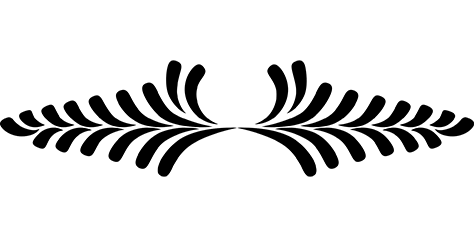
\includegraphics[width=0.1\textwidth]{ornamental}

		\end{center}
	%	\let\newpage\relax% Avoid following page break
		
	\end{titlepage}

	
\begin{ejercicio}{1}
	Escribe el vector cero en $M_{3x4}(\mathbb{R})$
\end{ejercicio}
		\begin{definition}[Matriz]
		Una \textbf{Matriz} es un arreglo rectangular de elementos de un campo $ \F(\R) $ de la forma
		\begin{equation*}
		A_{m,n} = 
		\begin{pmatrix}
		a_{1,1} & a_{1,2} & \cdots & a_{1,n} \\
		a_{2,1} & a_{2,2} & \cdots & a_{2,n} \\
		\vdots  & \vdots  & \ddots & \vdots  \\
		a_{m,1} & a_{m,2} & \cdots & a_{m,n} 
		\end{pmatrix}
		\end{equation*}
		A los elementos $ a_{i,j} $ con $ 1 \leq j \leq n $ y $ 1 \leq i \leq m $ se les llama entradas de la matriz, a las matrices las denotamos por $ \mathds{A} $ 				\textit{(letras mayúsculas)} y al conjunto de las matrices de mn se les denota por $ M_{m\times n}(\F) $
		
	\end{definition}
	De esta manera tenemos que el vector cero de la matriz de 3 renglones por 4 columnas es aquella cuyas entradas (todas) son 0 \textit{i. e. }
		\begin{equation*}
		A_{3x4} = 
		\begin{pmatrix}
		a_{1,1} & a_{1,2} & a_{1,3} & a_{1,4} \\
		a_{2,1} & a_{2,2} & a_{2,3} & a_{2,4} \\
		a_{3,1} & a_{3,2} & a_{3,3} & a_{3,4} 
		\end{pmatrix}
		= 
		\begin{pmatrix}
		0 & 0 & 0 & 0\\
		0 & 0 & 0 & 0 \\
		0 & 0 & 0 & 0
		\end{pmatrix}
		\end{equation*}
		
\begin{ejercicio}{2}
 Sea $V$ el conjunto de todas las funciones diferenciables definidas en $\mathbb{R}$. Muestre que $V$ es un espacio vectorial con las operaciones usuales de suma y multiplicación por un escalar para funciones. 
\end{ejercicio}

	Veamos que la derivada cumple las siguientes propiedades
	\begin{align*}
	(f(x) + g(x))' &= \lim_{h\to 0} \dfrac{f(x +h) + g(x + h) - (f(x) + g(x))}{h}\\
	& = \lim_{h\to 0} \dfrac{f(x+h) - f(x) + g(x+h) - g(x)}{h}\\
	&= \lim_{h\to 0} \dfrac{f(x+h)-f(x)}{h} + \lim_{h\to 0} \dfrac{g(x+h)-g(x)}{h}\\
	&=f'(x) + g'(x)
	\end{align*}
	Así hemos probado que la derivada abre sumas
	\begin{align*}
	(cf(x))' &= \lim_{h\to 0} \dfrac{cf(x + h) - cf(x)}{h}\\
	& = c\lim_{h\to 0} \dfrac{f(x+h)-f(x)}{h}\\
	&= cf'(x)
	\end{align*}
	De esta manera queda conolidado que en la función derivada, los escalares son sacados de la función
	
	\begin{align*}
	f'(x) &= \lim_{h\to 0} \dfrac{f(x + h) - f(x)}{h}\\
	& = \lim_{h\to 0} \dfrac{c-c}{h}\\
	&= 0
	\end{align*}
	\begin{center}
		Esto se vale para cualquier constante, en particular el 0
	\end{center}
	
 \begin{ejercicio}{3}
 	Prueba que el conjunto de las funciones pares en $\mathbb{R}$ es un espacio vectorial con suma y multiplicación por escalar usuales para funciones. Recuerde que una función es par si $\forall x \in Dom(f)$ entonces $f(-x) = f(x)$ 
 \end{ejercicio}
 	
 	Si tenemos en cuenta que $f(-t) + g(-t) = f(t) + g(t)$ y que si tenemos constantes siempre ocurre que $cf(-t) = cf(t) $ entonces ya hemos probado las dos primeras condiciones y para hallar el neutro basta con usar el 0 del cambo $(\R)$ para notar que también lo manda al 0 vector.\\
 	
\begin{ejercicio}{4}
	Sea $V$ el conjunto de pares ordenados de números reales. Si $(a_{1},a_{2})$ y $(b_{1},b_{2})$ son elementos de $V$ y $\alpha \in \mathbb{R}$, definamos la suma y multiplicación escalar de la siguiente manera:
	\begin{enumerate}
		\item[(i)] $(a_{1},a_{2}) + (b_{1},b_{2}) = (a_{1} + b_{1}, a_{2}b_{2})$ 
		\item[(ii)] $\alpha(a_{1},a_{2}) = (\alpha a_{1},a_{2})$.\\
	\end{enumerate}
	¿Es $V$ un espacio vectorial sobre $\mathbb{R}$ con estas operaciones?\\
\end{ejercicio}

No puede ser un espacio vectorial porque si tenemos que \[ 0(a_1, a_2) = (0, a_2)  \] para cumplir el cero vector, entonces se compliría para cualquier $a_2$ lo cual no es posible pues contradice la unicidad del cero.\\

\begin{ejercicio}{5}
	Determinar cuales de los siguientes conjuntos son subespacios de $\mathbb{R}^{3}$ bajo las operaciones de suma y multiplicación por un escalar usual.
\end{ejercicio}
\begin{definition}
	Sea $ \mathcal{U} $ un subconjunto de $ \mathcal{V}$ espacio vectorial sobre $ \F $ decimos que $ \mathcal{U} $ es un subespacio vectorial de $ \mathcal{V} $ si cumple lo siguiente
	
	\begin{enumerate}[i)]
		\item $ \vec{0}  \in \mathcal{U} $
		\item $ \forall \vec{u}, \vec{v} \in \mathcal{U} \implies \vec{u} + \vec{v} \in \mathcal{U} $
		\item Sea $ \alpha \in \F, \vec{u} \in \mathcal{U} \implies \alpha \* \vec{u} \in \mathcal{U} $
	\end{enumerate}
	   
\end{definition}

a) $W_{1} = \lbrace (a_{1},a_{2},a_{3}) \in \mathbb{R}^{3} \big\vert  a_{1}=3a_{2}$ y $a_{3}=-a_{2} \rbrace$

Veamos que $ W_{1} $ contiene a $ \vec{0} $ esto es que algún elemento en $ W_{1} = (0,0,0) $ por lo que 
	\begin{align*}
		(0,0,0) &= (a_{1},a_{2},a_{3}) && \text{Por $ \vec{0} \in \R^3 $}\\
		&= (3a_{2},a_{2},-a_{2}) && \text{Por $a_{1}=3a_{2}$ y $a_{3}=-a_{2}$}\\
		&= (3(0),(0),-(0)) && \text{Para cualquier $ a_2 $}\\
		&= (0,0,0)
	\end{align*}
	
Por otra parte comprobemos que la suma está dentro de $ W_1 $ 

Sean $ \hat{u} = (a_{1},a_{2},a_{3})  $ y $\hat{v} (b_{1},b_{2},b_{3})  \in W_1$ la suma de vectores se realiza entrada a entrada por lo que
\begin{align*}
	(a_{1},a_{2},a_{3}) + (b_{1},b_{2},b_{3}) &= (3a_{2},a_{2},-a_{2}) + (3b_{2},b_{2},-b_{2})\\
	&= (3 a_2 + 3b_2, a_2 + b_2, -a_2 - b_2)\\
	&= (3( a_2 + b_2), (a_2 + b_2), -(a_2 +b_2))
\end{align*}
 Y como $ a_1 + b_2 \in \R^3$ entonces $ \hat{u} + \hat{v} \in W_1 $ por lo que cumple $ II) $\\
 
 Finalmente veamos que si $ k \in R, \hat{u} \in W_1 \implies k\hat{u} \in W_1$
 
	\begin{align*}
		k(3a_2, a_2, -a_2) \in W_1\\
		(3ka_2, ka_2, -ka_2) \in W_1
	\end{align*}
	
	Por lo tanto cumple $ III) $ 
	
	\begin{center}
		$ \therefore W_1  $ es subespacio vectorial de $ \R^3 $
	\end{center}


b) $W_{2} = \lbrace (a_{1},a_{2},a_{3}) \in \mathbb{R}^{3} \big\vert  a_{1} = a_{3} + 2 \rbrace$

Veamos si $ \hat{0} \in W_2 $ si esto ocurriera entonces $ (0,0,0)  \in W_2$ l que significaría lo siguiente
\begin{align*}
	(0,0,0) &= (a_3 + 2, a_2, a_3) && \text{Por que deben ser iguales entrada a entrada}\\
	0 &= a_3 + 2\\
	0 &= a_2 \\
	0 &= a_3 
\end{align*}
Podemos observar que en esta situación, $ a_3 = -2 \land a_3 = 0 $ lo cual no es posible, dicha contradicción vino de suponer que $ \hat{0} \in W_2 $

\[ \therefore \hat{0} \notin W_2  \] 
\begin{center}
	por lo que $ W_2 $ \textbf{no} es subespacio vectorial de $ \R^3 $
\end{center}


\noindent c) $W_{3} = \lbrace (a_{1},a_{2},a_{3}) \in \mathbb{R}^{3} \big\vert  2a_{1} - 7a_{2} + a_{3} = 0 \rbrace$

Notemos que en la declaración de los elementos de $ W_3 $ podemos deducir que \[ a_3 = 7a_2 - 2 a_1 \] entonces $ \hat{u} \in W_3 \implies \hat{u} = (a_1, a_2, 7a_2 - 2a_1)  $

Veamos que para cumplir $ I) $ el vector cero debería estar en $ W_1 $ \textit{i.e.} 

\begin{align*}
	(0,0,0) &= (a_1, a_2, 7a_2 - 2 a_1) \\
	0 &=  a_1\\
	0 &=  a_2\\
	0 &=  7a_2 -2 a_1
\end{align*}
 lo anterior se cumple si $ a_2 = 0 = a_1 $
 
 $$ \therefore \hat{0} \in W_3 $$
 
 Ahora, sean $ \hat{u}, \hat{v} \in W_3 \implies \hat{u} = (a_1, a_2, 7a_2 - 2a_1) \land \hat{v} = (b_1, b_2, 7b_1 - 2 b_1) $ y probemos que $ \hat{u} + \hat{v} \in W_3 $
 
 \begin{align*}
 	(a_1, a_2, 7a_2 - 2a_1) + (b_1, b_2, 7b_1 - 2 b_1) &= (a_1 + b_1, a_2 + b _2, 7a_2 + 7b_2 -2a_1 - 2b_1)\\
 	&= (a_1 + b_1, a_2 + b _2, 7(a_2 + b_2) -2(a_1 +b_1))
 \end{align*}
 y como $ a_1 + b_1 \in R $ también se encontrarán dentro de $ W_3 $ por lo que la suma es cerrada en el conjunto $ W_3 $
 
 Por último veamos que si $ k \in \R, \hat{u} \in W_3 \implies k\* \hat{u} \in W_3 $
	\begin{align*}
		k\hat{u} &= k(a_1, a_2, 7a_2 - 2a_1)\\
		k\hat{u} &= (ka_1, ka_2, 7ka_2 - 2ka_1)
	\end{align*}
	De lo anterior podemos concluir que cada uno de esos $ ka_1, ka_2 $  elementos estarán en $ \R  $ por lo que $ k\hat{u} $ resultarán también estar en $ W_3 $
	\begin{center}
	$ \therefore W_3$ es un subespacio vectorial de $ \R^3 $
	\end{center}

d) $W_{4} = \lbrace (a_{1},a_{2},a_{3}) \in \mathbb{R}^{3} \big\vert  a_{1} - 4a_{2} - a_{3} = 0 \rbrace$
De la definición de los elementos de $ W_4 $ se sigue que si $ \hat{u} $ es un elemento de este conjunto, tendrá la forma $ \hat{u}= (4a_2 + a_3, a_2, a_3) $
Comencemos averiguando si $ W_4 $ tiene elemento neutro, \textit{i. e.}

\begin{align*}
	(0,0,0) &= (4a_2 + a_3, a_2, a_3) \\
	0 &= 4a_2 + a_3 && \text{para ser iguales entrada a entrada}\\
	0 &= a_2 && \\
	0 &= a_3 && 
\end{align*}
Lo anterior ocurre cuando $ a_2 = a_3 = 0 $ por lo que $ \hat{0} \in W_4 $ y así cumple la condición \textit{I)}

Siguiendo con la comprobación de sus propiedades como subespacio vectorial, tenemos que: Sean $ \hat{u}, \hat{v} \in W_4 \implies \hat{u} + \hat{v} \in W_4 $ \textit{i. e.}

\begin{align*}
		\hat{u} + \hat{v} &= (4a_2 + a_3, a_2, a_3) + (4b_2 + b_3, b_2, b_3)\\
		&= (4a_2 + 4b_2 + b_3 + a_3, a_2 + b_2, a_3 + b_3) && \text{sumando entrada por entrada}\\
		&= (4(a_2 + b_2) + (b_3 + a_3), (a_2 + b_2), (a_3 + b_3)) && \text{asociatividad y distributividad en $ \R $}\\
\end{align*}
y como $ (a_2 + b_2) \in \R $ la suma de $ \hat{u}, \hat{v} \in W_4 $

Finalmente notemos que si $ k \in \R, \hat{u} \in W_4 \implies k\* \hat{u} \in W_4 $ 

\begin{align*}
	k\hat{u} & = k(4a_2 + a_3, a_2, a_3)\\
	 & = (4ka_2 + ka_3, ka_2, ka_3) && \text{por distributividad}
\end{align*}

y $ ka_2, k_3 \in \R $ entonces $ k\*\hat{u} \in W_4 $
\begin{center}
	$ \therefore W_4 $ es subespacio vectorial de $ \R^3 $
\end{center}


\begin{ejercicio}{6}
	En cada caso diga si los vectores son generados por el conjunto $S$
\end{ejercicio}

\begin{definition}
	Sea $ \mathcal{S} $ un subconjunto de un espacio vectorial $ \mathcal{V} $ decimos que $ \mathcal{S} $ genera a $ \mathcal{V} $ si $ \forall \hat{x} \in \mathcal{V} $ es una combinación lineal de elementos de $ \mathcal{S} $ al generado de s se le denota como $ span(\mathcal{S}), <\mathcal{S}>, gen(\mathcal{S})$ 
\end{definition}

\textbf{a)} $(2,-1,1), S =  \lbrace (1,0,2),(-1,1,1) \rbrace$

Sea $\alpha _1$, $\alpha _2 \in \mathbb{R}$.

Entonces $(2,-1,1) = \alpha _{1}(1,0,2) + \alpha _{2}(-1,1,1) = (\alpha _{1}, 0, 2\alpha _{1})+ (-\alpha _{2},\alpha _{2},\alpha _{2}) = \alpha _{1}-\alpha _{2},\alpha _{2},2\alpha _{1}+\alpha _{2}$.

Tenemos el siguiente sistema de ecuaciones:
	\begin{align*}
		\alpha_{1}-\alpha_{2}&= 2 \\
		\alpha_{2} &= -1\\
		2\alpha_{1}+\alpha_{2}&=1\\
	\end{align*}
	Ahora:
	\begin{align*}
		\alpha_{1} -(-1)&=2 \\
		\alpha_{2}&=-1\\
		2\alpha_{1} + \alpha_{2} &= 1\\
	\end{align*}
Al resolver el sistema, obtenemos:
	\begin{align*}
		\alpha_{1}&=1 \\
		\alpha_{2} &= -1 \\
		1 &= 1
	\end{align*}
Entonces:\\ $1(1,0,2) + (-1)(-1,1,1) = (1,0,2) + (1,-1,-1) = (2,-1,1)$\\
Cómo el sistema de ecuaciones si se satisface, el conjunto $S$ SI genera al vector $(2,-1,-1)$\\ \\

\noindent \textbf{b)} $(2,-1,1,3), S =  \lbrace (1,0,1,-1),(0,1,1,1) \rbrace$

Sea $\alpha _1$, $\alpha _2 \in \mathbb{R}$.\\
Entonces: $(2,-1,1,3)=\alpha_{1}(1,0,1,-1)+\alpha_{2}(0,1,1,1)= (\alpha_{1},0,\alpha_{1},-\alpha_{1})+(0,\alpha_{2},\alpha_{2},\alpha_{2})= \alpha_{1},\alpha_{2},\alpha_{1}+\alpha_{2},-\alpha_{1}+\alpha_{2}$.\\
Tenemos el siguiente sistema de ecuaciones:\\
	\begin{align*}
		\alpha_{1}=2\\
		\alpha_{2} = -1\\
		\alpha_{1}+\alpha_{2}=1\\
		-\alpha_{1}+\alpha_{2}=3
	\end{align*}
	Ahora:
	\begin{align*}
		\alpha_{1}=2\\
		\alpha_{2}= -1\\
		2-1  =1\\
		-(-1)+2 = 3\\
	\end{align*}
	Por último:
	\begin{align*}
		\alpha_{1}=2\\
		\alpha_{2}=-1\\
		1=1\\
		3=3
	\end{align*}
Al resolver el sistema de ecuaciones verificamos si el conjunto $S$ genera al vector. Entonces:
\[2(1,0,1,-1)+(-1)(0,1,1,1)=(2,0,2,-2)+(0,-1,-1,-1)=(2,-1,-1,-3)\]
Como el producto de los escalares por los elementos del conjunto $S$ no forman al vector, podemos concluir que $S$ \textbf{NO} genera a $(2,-1,1,3)$.\\

\textbf{c)} $2x^3 - x^2 + x + 3, S =  \lbrace x^3 + x^2 + x +1, x^2 + x +1, x +1 \rbrace$\\

Sean $\alpha_1 $, $\alpha_2$ y $\alpha_3$ elementos del campo, si suponemos que $2x^3 - x^2 + x + 3$ es generado por $S$ implicará que existen dichos 3 elementos $\tq$ 
\[ 2x^3 - x^2 + x + 3 = \alpha_1 (x^3 + x^2 + x +1) + \alpha_2 (x^2 + x +1) + \alpha_3 (x +1) \]

	\begin{align*}
		\alpha_1 x^3 + \alpha_1 x^2 + \alpha_1 x + \alpha_1 	\\
		\alpha_2 x^2 + \alpha_2 x + \alpha_2 \\
		\alpha_3 x + \alpha_3 
	\end{align*}
Por lo que ocurre lo siguiente
\[ 2x^3 - x^2 + x + 3 = \alpha_1 x^3 + \alpha_1 x^2 + \alpha_1 x + \alpha_1 + \alpha_2 x^2 + \alpha_2 x + \alpha_2 +\alpha_3 x + \alpha_3  \]
	\begin{align*}
		2x^3 - x^2 + x + 3 &= \alpha_1 x^3 + \alpha_1 x^2 + \alpha_1 x + \alpha_1 + \alpha_2 x^2 + \alpha_2 x + \alpha_2 +\alpha_3 x + \alpha_3 \\
		 &= x^3 (\alpha_3)  + x^2 (\alpha_2 + \alpha_1) + x(\alpha_3 + \alpha_2 + \alpha_1) + \alpha_1 + \alpha_2 + \alpha_3
	 \end{align*}
	\begin{align*}
		\alpha_3 &=  2\\
		\alpha_2 &= -1 - \alpha_1 \\
		\alpha_2 &= -1 - 2\\
		\alpha_2 &= -3
	\end{align*}

Ahora llegamos a una contradicción, puesto que el sistema de ecuaciones anterior implica que $\alpha_1 + \alpha_2 + \alpha_3 = 3 = 1$ por lo que el conjunto S no genera $ 2x^3 - x^2 + x + 3$

\textbf{d)} $$ \begin{pmatrix} 1 & 2 \\ -3 & 4 \end{pmatrix},  S =  \left\lbrace \begin{pmatrix} 1 & 0 \\ -1 & 0 \end{pmatrix} , \begin{pmatrix} 0 & 1 \\ 0 &1 \end{pmatrix} , \begin{pmatrix} 1 & 1 \\ 0 &0 \end{pmatrix} \right\rbrace$$
Recordemos que la suma de matrices se hace entrada por entrada eso es, si se van a sumar 2 matrices $A + B$ se hace de la forma $a_{ij} + b_{ij}  \forall i,j \in A,B$ de tal manera que existen  $a_{ij} + b_{ij}  \forall i,i \in A,B$ de tal manera que existen $\alpha, \beta, \gamma \tq $

\begin{align*}
 \begin{pmatrix} 
 1 & 2 \\ 
 -3 & 4 
 \end{pmatrix} &= \alpha \begin{pmatrix} 
 1 & 0 \\ 
 -1 & 0 
 \end{pmatrix}  + \beta \begin{pmatrix} 
 0 & 1 \\
 0 &1 
 \end{pmatrix}  + \gamma  \begin{pmatrix} 
 1 & 1 \\
 0 &0 
 \end{pmatrix} \\
  & = \begin{pmatrix} \alpha_{1,1}  + \gamma_{1,1} & \beta_{1,2} + \gamma_{1,2} \\ -\alpha_{2,1} & \beta_{2,2} \end{pmatrix}  
\end{align*}

Notemos que $$ -\alpha_{2,1} = -3  \implies  \alpha = 3$$ y luego 
$$\beta_{2,2} = 4 \implies \beta = 4 $$ y finalmente $$\gamma = 2 - \beta_{1,2} \implies \gamma = 4 $$

\begin{ejercicio}{7}
	Determina cuando los siguientes conjuntos son linealmente dependientes o linealmente independientes.
\end{ejercicio}


\textbf{a)} $\left \lbrace \begin{pmatrix} 1 & -3 \\ -2 & 4 \end{pmatrix} , \begin{pmatrix} -2 & 6 \\ 4 & -8 \end{pmatrix} \right \rbrace \in M_{2x2}(\mathbb{R})$\\

Sean $\alpha _1, \alpha _2, \in \mathbb{R}$. Entonces:\\

$$\alpha_1 \begin{pmatrix} 1 & -3 \\ -2 & 4 \end{pmatrix}  + \alpha_2 \begin{pmatrix} -2 & 6 \\ 4 & -8 \end{pmatrix} = \begin{pmatrix}
0 & 0 \\ 0 & 0 \end{pmatrix}$$

Ahora:
$$\begin{pmatrix} \alpha_1 & -3\alpha_{1} \\ -2\alpha_{1} & 4\alpha_{1} \end{pmatrix} +
\begin{pmatrix} -2\alpha_{2} & 6\alpha_2 \\ 4\alpha_{2} & -8\alpha_{2} \end{pmatrix} = \begin{pmatrix} 	0 & 0 \\ 0 & 0 \end{pmatrix}$$

Sumamos cada elemento de las matrices al correspondiente reglón y columna:\\
		$$\begin{pmatrix}
		\alpha_{1}-2\alpha_{2} & -3\alpha_{1}+6\alpha_{2} \\ -2\alpha_{1}+4\alpha_{2} & 4\alpha_{1}-8\alpha_{2}
		\end{pmatrix} = \begin{pmatrix}
		0 & 0 \\ 0 & 0
		\end{pmatrix}$$

Tenemos el siguiente sistema de ecuaciones:
	\begin{align*}
		\alpha_{1}-2\alpha_{2} = 0\\
		-3\alpha_{1} + 6\alpha_{2} = 0\\
		-2\alpha_{1}+4\alpha_{2}= 0\\
		4\alpha_{1}-8\alpha_{2}= 0
	\end{align*}
Multiplicamos dos veces el renglón 3 y lo sumamos al renglón 4. También multiplicamos dos veces el renglón 1 y lo sumamos al renglón 3.
\begin{align*}	
	\alpha_{1}-2\alpha_{2} &= 0\\
	-3\alpha_{1}+6\alpha_{2}&= 0\\
	0\alpha_{1}+0\alpha_{2}&=0\\
	0\alpha_{1}+0\alpha_{2}&= 0
\end{align*}
Por último multiplicamos tres veces el renglón 1 y lo sumamos al renglón 2:
\begin{align*}
	\alpha_{1}-2\alpha_{2}=0\\
	0\alpha_{1}+0\alpha_{2}=0
\end{align*}	

Entonces $\alpha_{1}=2\alpha_{2}$.\\ Esto indica que $\alpha_{1}$ depende de $\alpha_{2}$. Por lo tanto, el conjunto  $\begin{pmatrix} 1 & -3 \\ -2 & 4 \end{pmatrix} , \begin{pmatrix} -2 & 6 \\ 4 & -8 \end{pmatrix}\in M_{2x2}$  es \textbf{linealmente dependiente}.

\textbf{b)} $\left \lbrace \begin{pmatrix} 1 & -2 \\ -1 & 4 \end{pmatrix} ,\begin{pmatrix} -1 & 1 \\ 2 & -4 \end{pmatrix}  \right \rbrace \in M_{2x2}(\mathbb{R})$\\

Sean $\alpha _1, \alpha _2, \in \mathbb{R}$. Entonces:

$$\alpha_1 \begin{pmatrix} 1 & -2 \\ -1 & 4 \end{pmatrix}  + \alpha_2 \begin{pmatrix} -1 & 1 \\ 2 & -4 \end{pmatrix} = \begin{pmatrix}
0 & 0 \\ 0 & 0 \end{pmatrix}$$

Ahora:
$$\begin{pmatrix} \alpha_1 & -2\alpha_{1} \\ -\alpha_{1} & 4\alpha_{1} \end{pmatrix} +
\begin{pmatrix} -\alpha_{2} & \alpha_2 \\ 2\alpha_{2} & -4\alpha_{2} \end{pmatrix} = \begin{pmatrix} 	0 & 0 \\ 0 & 0 \end{pmatrix}$$

Sumamos cada elemento de las matrices al correspondiente reglón y columna:\\

\begin{center}
	$\begin{pmatrix}
	\alpha_{1}-\alpha_{2} & -2\alpha_{1}+\alpha_{2} \\ -\alpha_{1}+2\alpha_{2} & 4\alpha_{1}-4\alpha_{2}
	\end{pmatrix} = \begin{pmatrix}
	0 & 0 \\ 0 & 0
	\end{pmatrix}$
\end{center}

Tenemos el siguiente sistema de ecuaciones:
	\begin{align*}
	\alpha_{1}-\alpha_{2} &= 0\\
	-2\alpha_{1} + \alpha_{2} &= 0\\
	-\alpha_{1}+2\alpha_{2}&= 0\\
	4\alpha_{1}-4\alpha_{2}&= 0
	\end{align*}

Multiplicamos cuatro veces el renglón 1 y lo restamos al renglón 4. También sumamos el renglón 1 al renglón 2:
	\begin{align*}
	\alpha_{1}-\alpha_{2} &= 0\\
	-2\alpha_{1} + \alpha_{2} &= 0\\
	0\alpha_{1}+\alpha_{2}&= 0\\
	0\alpha_{1}+0\alpha_{2}&= 0
	\end{align*}
Tenemos que $\alpha_{2}= 0$, Entonces lo sustituimos en las demás ecuaciones:
	\begin{align*}
	\alpha_{1}-0 &= 0\\
	-2\alpha_{1} + 0 &= 0\\
	\end{align*}
Es claro notar que $\alpha_{1}=0$ y $\alpha_{2}=0$.\\ Cómo ambos valen 0, podemos concluir que el conjunto $\begin{pmatrix} 1 & -2 \\ -1 & 4 \end{pmatrix} ,\begin{pmatrix} -1 & 1 \\ 2 & -4 \end{pmatrix}\in M_{2x2}(\mathbb{R})$ es \textbf{linealmente independiente}.

\textbf{c)} $\lbrace x^{3} + 2x^{2}, -x^{2} + 3x + 1, x^{3} - x^{2} + 2x -1 \rbrace \in P_{3}(\mathbb{R})$ \\

Sean $\alpha_{1}, \alpha_{2}, \alpha_{3}\in \mathbb{R}$.

Tenemos que: $0x^{3}+0x^{2}+0x+d = \alpha_{1}(x^{3}+2x^{2})+ \alpha_{2}(-x^{2}+3x+1)+ \alpha_{3}(x^{3}-x^{2}+2x-1)$ \\  
        
 $x^{3}+0x^{2}+0x+0=(\alpha_{1}+\alpha_{3})x^{3}+(2\alpha_{1}-\alpha_{2}-\alpha_{3})x^{2}+(3\alpha_{2}+2\alpha_{3})x+(\alpha_{2}-\alpha_{3})$.
 
 Obtenemos el siguiente sistema de ecuaciones:
 	\begin{align*}
 	\alpha_{1}+0\alpha_{2}+\alpha_{3}&=0\\
 	2\alpha_{1}-\alpha_{2}-\alpha_{3}&=0\\
 	0\alpha_{1}+3\alpha_{2}+2\alpha_{3}&=0\\
 	0\alpha_{1}+\alpha_{2}-\alpha_{3}&=0
 	\end{align*}

Ahora multiplicamos -3 veces el renglón 4 y le sumamos el renglón 1:
	\begin{align*}
	\alpha_{1}+0\alpha_{2}+\alpha_{3}&=0\\
	2\alpha_{1}-\alpha_{2}-\alpha_{3}&=0\\
	0\alpha_{1}+3\alpha_{2}+2\alpha_{3}&=0\\
	0\alpha_{1}+0\alpha_{2}+5\alpha_{3}&=0
	\end{align*}
Podemos obtener que $\alpha_{3}=0$. Entonces sustituimos este valor en las ecuaciones.
	\begin{align*}
	\alpha_{1}+0\alpha_{2}+0&=0\\
	2\alpha_{1}-\alpha_{2}-0&=0\\
	0\alpha_{1}+3\alpha_{2}+0&=0\\
	\alpha_{3}&=0
	\end{align*}

De lo anterior deducimos que $\alpha_{1}= 0$, por tanto:
	\begin{align*}
	0-\alpha_{2}-0&=0\\
	0+3\alpha_{2}+0&=0\\
	\alpha_{3}&=0
	\end{align*}

Entonces $\alpha_{1}=0$, $\alpha_{2}=0$, $\alpha_{3}=0$. Podemos que concluir que el conjunto $\lbrace x^{3} + 2x^{2}, -x^{2} + 3x + 1, x^{3} - x^{2} + 2x -1 \rbrace \in P_{3}(\mathbb{R})$ es \textbf{linealmente independiente}.\\

\textbf{d)} $\lbrace (1,-1,2), (1,-2,1), (1,1,4) \rbrace \in \mathbb{R}^{3}$\\

Sean $\alpha_{1}, \alpha_{2}, \alpha_{3}\in \mathbb{R}$. Entonces:

$\alpha_{1}(1,-1,2)+\alpha_{2}(1,-2,1)+ \alpha_{3}(1,1,4)=(0,0,0)$.
Ahora:\\

$(\alpha_{1},-\alpha_{1},2\alpha_{1})+(\alpha_{2},-2\alpha_{2},\alpha_{2})+ (\alpha_{3},\alpha_{3},4\alpha_{3})=(0,0,0)$. Ordenamos los escalares:\\

$(\alpha_{1}+\alpha_{2}+\alpha_{3}, -\alpha_{1}-2\alpha_{2}+\alpha_{3}, 2\alpha_{1}+\alpha_{2}+4\alpha_{3})= (0,0,0)$\\

Obtenemos el siguiente sistema de ecuaciones:
\begin{center}
	\begin{align*}
	\alpha_{1}+\alpha_{2}+\alpha_{3}=0\\
	-\alpha_{1}-2\alpha_{2}+\alpha_{3}=0\\
	2\alpha_{1}+\alpha_{2}+4\alpha_{3}=0
	\end{align*}
\end{center}

Multiplicamos dos veces el renglón 1 y lo sumamos a "menos" el renglón 3. También sumamos el renglón 1 al renglón 2.
\begin{center}
	\begin{align*}
	\alpha_{1}+\alpha_{2}+\alpha_{3}=0\\
	0\alpha_{1}-\alpha_{2}+2\alpha_{3}=0\\
	0\alpha_{1}+\alpha_{2}-2\alpha_{3}=0
	\end{align*}
\end{center}

Ahora al renglón 3 le sumamos el renglón 2. Y al renglón 1 le sumamos el renglón 2.
\begin{center}
	\begin{align*}
	\alpha_{1}+0\alpha_{2}+3\alpha_{3}=0\\
	0\alpha_{1}-\alpha_{2}+2\alpha_{3}=0\\
	0\alpha_{1}+0\alpha_{2}-0\alpha_{3}=0
	\end{align*}
\end{center}

Entonces nos queda el siguiente sistema.
\begin{center}
	\begin{align*}
	\alpha_{1}+3\alpha_{3}=0\\
	-\alpha_{2}+2\alpha_{3}=0
	\end{align*}
\end{center}

De esto podemos deducir que $\alpha_{1}=-3\alpha_{3}$, $\alpha_{2}= 2\alpha_{3}$ y $\alpha_{3}= \frac{\alpha_{2}}{2}$.\\

Entonces podemos concluir que el conjunto $\lbrace (1,-1,2), (1,-2,1), (1,1,4) \rbrace \in \mathbb{R}^{3}$ es \textbf{linealmente dependiente}.\\

\textbf{e)}$\lbrace (1,-1,2), (2,0,1),(-1,2,-1)\rbrace \in \mathbb{R}^{3}$\\

Sean $\alpha_{1}, \alpha_{2}, \alpha_{3}\in \mathbb{R}$.

\begin{align*}
	\alpha_{1}(1,-1,2)+\alpha_{2}(2,0,1)+ \alpha_{3}(-1,2,-1)&=(0,0,0) && \text{Ahora}\\
	(\alpha_{1},-\alpha_{1},2\alpha_{1})+(2\alpha_{2},0\alpha_{2},\alpha_{2})+ (-\alpha_{3},2\alpha_{3},-\alpha_{3})&=(0,0,0) && \text{Ordenamos los escalares}\\
	(\alpha_{1}+2\alpha_{2}-\alpha_{3}, -\alpha_{1}+0\alpha_{2}+2\alpha_{3}, 2\alpha_{1}+\alpha_{2}-\alpha_{3}) &= (0,0,0) &&\\
\end{align*}

Obtenemos el siguiente sistema de ecuaciones:
\begin{center}
	\begin{align*}
	\alpha_{1}+2\alpha_{2}-\alpha_{3}=0\\
	-\alpha_{1}+0\alpha_{2}+2\alpha_{3}=0\\
	2\alpha_{1}+\alpha_{2}-\alpha_{3}=0
	\end{align*}
\end{center}

Primero multiplicamos dos veces el renglón 1 y lo restamos al renglón 3. Luego sumamos el renglón 2 al renglón 1.
\begin{center}
	\begin{align*}
	0\alpha_{1}+2\alpha_{2}+\alpha_{3}=0\\
	-\alpha_{1}+0\alpha_{2}+2\alpha_{3}=0\\
	0\alpha_{1}+3\alpha_{2}-\alpha_{3}=0
	\end{align*}
\end{center}

Ahora al renglón 3 le sumamos el renglón 1:

\begin{center}
	\begin{align*}
	0\alpha_{1}+2\alpha_{2}+\alpha_{3}=0\\
	-\alpha_{1}+0\alpha_{2}+2\alpha_{3}=0\\
	0\alpha_{1}+5\alpha_{2}-0\alpha_{3}=0
	\end{align*}
\end{center}

De lo anterior obtenemos que $\alpha_{2}= 0$ y sustituimos en las demás ecuaciones.

\begin{center}
	\begin{align*}
	0+\alpha_{3}=0\\
	-\alpha_{1}+2\alpha_{3}=0\\
	\alpha_{2}=0
	\end{align*}
\end{center}

Es fácilmente apreciar que $\alpha_{1}=0$, $\alpha_{2}=0$ y $\alpha_{3}=0$\\

Por lo tanto, podemos concluir que el conjunto $ (1,-1,2), (2,0,1),(-1,2,-1) \in \mathbb{R}^{3}$ es \textbf{linealmente independiente}\\

Recuerde que $P_{n}(\mathbb{R}) = \{ a_0 +  a_1x +  a_2x^2 + \cdots +  a_n x^n \big\vert a_k \in \mathbb{R} \,  \forall k = 0,1,2,\dots n\}$
\\

\begin{ejercicio}{8}
	¿Cuáles de los siguientes conjuntos son bases para $\mathbb{R}^{3}$?
\end{ejercicio}
	\begin{definition}
		Una \textbf{base} $ \beta $ de $ \mathcal{V} $ espacio vectorial es un subconjunto de $ \mathcal{V} \tq \beta$  genera a $ \mathcal{V} $ y $ \beta $ es linealmente independiente
	\end{definition}

	a)  $S = \lbrace (1,0,-1),(2,5,1),(0,-4,3) \rbrace$
	En primer lugar veamos quién es el generado del conjunto $ S $, recordemos que un conjunto genera a otro $ \forall \hat{x} \in \mathcal{V} $ es una combinación lineal de elementos de $ \mathcal{S} $ 
	
	Sean $ \alpha, \beta, \gamma \in \R $ entonces
	\[ \alpha(1,0,-1) + \beta(2,5,1) + \gamma(0,-4,3)  \]
	\begin{align*}
		\alpha(1,0,-1)+ \beta(2,5,1)+ \gamma(0,-4,3) & = (\alpha,0,-\alpha) + (2\beta,5\beta,\beta) + (0,-4\gamma,3\gamma)\\
		& = (\alpha + 2\beta ,5\beta -4\gamma,-\alpha + \beta +3\gamma)
	\end{align*}
	Necesitamos que cada uno de esos vectores pueda ser el valor de una posición de $ \R^3 $ por lo que debería verse como \[ 	\alpha(1,0,-1)+ \beta(2,5,1)+ \gamma(0,-4,3) = \delta(1,0,0) + \epsilon(0,1,0) + \eta(0,0,1) \] De esta manera podemos obtener el siguiente sistema de ecuaciones
	\begin{align*}
		\alpha + 2\beta + 0\gamma = \delta + 0\epsilon + 0\eta\\
		0\alpha + 5\beta -4\gamma = 0\delta + \epsilon + 0\eta\\
		-\alpha + \beta +3\gamma = 0\delta +0\epsilon + \eta
	\end{align*}
	\begin{align*}
		\begin{pmatrix}
			\alpha & 2\beta & 0\gamma\\
			0\alpha & 5\beta & -4\gamma\\
			-\alpha & \beta & 3\gamma
		\end{pmatrix}
		&= 		\begin{pmatrix}
		\delta & 0\epsilon & 0\eta\\
		0\delta & \epsilon & 0\eta\\
		0\delta & 0\epsilon & \eta
		\end{pmatrix}  = 		 \begin{pmatrix}[ccc|ccc]
		\alpha & 2\beta & 0\gamma & \delta & 0\epsilon & 0\eta\\
		0\alpha & 5\beta & -4\gamma& 0\delta & \epsilon & 0\eta\\
		-\alpha & \beta & 3\gamma & 0\delta & 0\epsilon & \eta
		\end{pmatrix} 
	\end{align*}
	\begin{align*}
		 \begin{pmatrix}[ccc|ccc]
		 \alpha & 2\beta & 0\gamma & \delta & 0\epsilon & 0\eta\\
		 0\alpha & 5\beta & -4\gamma& 0\delta & \epsilon & 0\eta\\
		 -\alpha & \beta & 3\gamma & 0\delta & 0\epsilon & \eta
		 \end{pmatrix} &= 		 \begin{pmatrix}[ccc|ccc]
		 \alpha & 2\beta & 0\gamma & \delta & 0\epsilon & 0\eta\\
		 0\alpha & 5\beta & -4\gamma& 0\delta & \epsilon & 0\eta\\
		 0\alpha & 3\beta & 3\gamma & \delta & 0\epsilon & \eta
		 \end{pmatrix} && \text{1ra fila + 2da fila en \textbf{3ra fila}} \\
		 \begin{pmatrix}[ccc|ccc]
		 \alpha & 2\beta & 0\gamma & \delta & 0\epsilon & 0\eta\\
		 0\alpha & 5\beta & -4\gamma& 0\delta & \epsilon & 0\eta\\
		 0\alpha & 3\beta & 3\gamma & \delta & 0\epsilon & \eta
		 \end{pmatrix} &= \begin{pmatrix}[ccc|ccc]
		 \alpha & 2\beta & 0\gamma & \delta & 0\epsilon & 0\eta\\
		 0\alpha & 1\beta & -\frac{4}{5}\gamma& 0\delta & \frac{1}{5}\epsilon & 0\eta\\
		 0\alpha & 3\beta & 3\gamma & \delta & 0\epsilon & \eta
		 \end{pmatrix} && \text{2da fila $ \* \frac{1}{5} $ en \textbf{2da fila}}\\
		 \begin{pmatrix}[ccc|ccc]
		 \alpha & 2\beta & 0\gamma & \delta & 0\epsilon & 0\eta\\
		 0\alpha & 1\beta & -\frac{4}{5}\gamma& 0\delta & \frac{1}{5}\epsilon & 0\eta\\
		 0\alpha & 3\beta & 3\gamma & \delta & 0\epsilon & \eta
		 \end{pmatrix} &= \begin{pmatrix}[ccc|ccc]
		 \alpha & 2\beta & 0\gamma & \delta & 0\epsilon & 0\eta\\
		 0\alpha & 1\beta & -\frac{4}{5}\gamma& 0\delta & \frac{1}{5}\epsilon & 0\eta\\
		 0\alpha & 0\beta & \frac{27}{5}\gamma & \delta & -\frac{3}{5}\epsilon & \eta
		 \end{pmatrix} && \text{2da fila $ \* -3  +  3^{ra}$ fila en \textbf{3ra fila}}\\
		 \begin{pmatrix}[ccc|ccc]
		 \alpha & 2\beta & 0\gamma & \delta & 0\epsilon & 0\eta\\
		 0\alpha & 1\beta & -\frac{4}{5}\gamma& 0\delta & \frac{1}{5}\epsilon & 0\eta\\
		 0\alpha & 0\beta & \frac{27}{5}\gamma & \delta & -\frac{3}{5}\epsilon & \eta
		 \end{pmatrix} & = \begin{pmatrix}[ccc|ccc]
		 \alpha & 2\beta & 0\gamma & \delta & 0\epsilon & 0\eta\\
		 0\alpha & 1\beta & -\frac{4}{5}\gamma& 0\delta & \frac{1}{5}\epsilon & 0\eta\\
		 0\alpha & 0\beta & \gamma & \frac{5}{27}\delta & -\frac{1}{9}\epsilon & \frac{5}{27}\eta
		 \end{pmatrix} && \text{ 3ra fila $ \* \frac{5}{27}$ \textbf{en 3ra fila} }\\
		 \begin{pmatrix}[ccc|ccc]
		 \alpha & 2\beta & 0\gamma & \delta & 0\epsilon & 0\eta\\
		 0\alpha & 1\beta & -\frac{4}{5}\gamma& 0\delta & \frac{1}{5}\epsilon & 0\eta\\
		 0\alpha & 0\beta & \gamma & \frac{5}{27}\delta & -\frac{1}{9}\epsilon & \frac{5}{27}\eta
		 \end{pmatrix} &= \begin{pmatrix}[ccc|ccc]
		 \alpha & 2\beta & 0\gamma & \delta & 0\epsilon & 0\eta\\
		 0\alpha & 1\beta & 0\gamma& \frac{4}{27}\delta & \frac{1}{9}\epsilon & \frac{4}{27}\eta\\
		 0\alpha & 0\beta & \gamma & \frac{5}{27}\delta & -\frac{1}{9}\epsilon & \frac{5}{27}\eta
		 \end{pmatrix} && \text{(3ra fila $ \* \dfrac{4}{5}) + 2^{da} $  fila \textbf{en 2da fila} }\\
		 \begin{pmatrix}[ccc|ccc]
		 \alpha & 2\beta & 0\gamma & \delta & 0\epsilon & 0\eta\\
		 0\alpha & 1\beta & 0\gamma& \frac{4}{27}\delta & \frac{1}{9}\epsilon & \frac{4}{27}\eta\\
		 0\alpha & 0\beta & \gamma & \frac{5}{27}\delta & -\frac{1}{9}\epsilon & \frac{5}{27}\eta
		 \end{pmatrix} & = \begin{pmatrix}[ccc|ccc]
		 \alpha & 0\beta & 0\gamma & \frac{19}{27}\delta & -\frac{2}{9}\epsilon & -\frac{8}{27}\eta\\
		 0\alpha & 1\beta & 0\gamma& \frac{4}{27}\delta & \frac{1}{9}\epsilon & \frac{4}{27}\eta\\
		 0\alpha & 0\beta & \gamma & \frac{5}{27}\delta & -\frac{1}{9}\epsilon & \frac{5}{27}\eta
		 \end{pmatrix} && \text{(2da fila $ \* -2) + 1^{a} $ fila \textbf{en 1ra fila}}\\
		 \begin{pmatrix}[ccc|ccc]
		 \alpha & 0\beta & 0\gamma & \frac{19}{27}\delta & -\frac{2}{9}\epsilon & -\frac{8}{27}\eta\\
		 0\alpha & 1\beta & 0\gamma& \frac{4}{27}\delta & \frac{1}{9}\epsilon & \frac{4}{27}\eta\\
		 0\alpha & 0\beta & \gamma & \frac{5}{27}\delta & -\frac{1}{9}\epsilon & \frac{5}{27}\eta
		 \end{pmatrix} & = \begin{pmatrix}[ccc|ccc]
		 1 & 0 & 0 & \frac{19}{27} & -\frac{2}{9} & -\frac{8}{27}\\
		 0 & 1 & 0& \frac{4}{27} & \frac{1}{9} & \frac{4}{27}\\
		 0 & 0 & 1 & \frac{5}{27} & -\frac{1}{9} & \frac{5}{27}
		 \end{pmatrix} && \text{Conservando sólo \textbf{coeficientes}}
	\end{align*}
	\begin{align*}
		\alpha &= \frac{19}{27}\delta -\frac{2}{9}\epsilon -\frac{8}{27}\eta\\
		\beta &= \frac{4}{27}\delta+ \frac{1}{9}\epsilon + \frac{4}{27}\eta\\
		\delta &= \frac{5}{27}\delta -\frac{1}{9}\epsilon+ \frac{5}{27}\eta
	\end{align*}
	\[ \therefore  \mathcal{S} \text{ genera a } \R^3  \]
	
	Ahora veamos si es linealmente independiente, lo cual ocurre si la única solución para \[ \alpha(1,0,-1) + \beta(2,5,1) + \gamma(0,-4,3) = 0  \] es que \[ \alpha = \beta = \gamma = 0 \]
	
		\begin{align*}
		\alpha + 2\beta + 0\gamma =0\\
		0\alpha + 5\beta -4\gamma = 0\\
		-\alpha + \beta +3\gamma = 0
		\end{align*}
	Resolviendo dicho sistema obtenemos que 
	
		\begin{align*}
		\begin{pmatrix}[ccc|c]
		\alpha & 2\beta & 0\gamma & 0\\
		0\alpha & 5\beta & -4\gamma& 0\\
		-\alpha & \beta & 3\gamma & 0
		\end{pmatrix} &= \begin{pmatrix}[ccc|ccc]
		\alpha & 2\beta & 0\gamma & 0\\
		0\alpha & 5\beta & -4\gamma& 0\\
		0\alpha & 3\beta & 3\gamma & 0
		\end{pmatrix} && \text{1ra fila + 2da fila en \textbf{3ra fila}} \\
		\begin{pmatrix}[ccc|ccc]
		\alpha & 2\beta & 0\gamma & 0\\
		0\alpha & 5\beta & -4\gamma& 0\\
		0\alpha & 3\beta & 3\gamma & 0
		\end{pmatrix} &= \begin{pmatrix}[ccc|ccc]
		\alpha & 2\beta & 0\gamma & 0\\
		0\alpha & 1\beta & -\frac{4}{5}\gamma& 0\\
		0\alpha & 3\beta & 3\gamma & 0
		\end{pmatrix} && \text{2da fila $ \* \frac{1}{5} $ en \textbf{2da fila}}\\
		\end{align*}
		\begin{align*}
		\begin{pmatrix}[ccc|ccc]
		\alpha & 2\beta & 0\gamma & 0\\
		0\alpha & 1\beta & -\frac{4}{5}\gamma& 0\\
		0\alpha & 3\beta & 3\gamma & 0
		\end{pmatrix} &= \begin{pmatrix}[ccc|ccc]
		\alpha & 2\beta & 0\gamma & 0\\
		0\alpha & 1\beta & -\frac{4}{5}\gamma& 0\\
		0\alpha & 0\beta & \frac{27}{5}\gamma & 0
		\end{pmatrix} && \text{2da fila $ \* -3  +  3^{ra}$ fila en \textbf{3ra fila}}\\
		\begin{pmatrix}[ccc|ccc]
		\alpha & 2\beta & 0\gamma 0\\
		0\alpha & 1\beta & -\frac{4}{5}\gamma& 0\\
		0\alpha & 0\beta & \frac{27}{5}\gamma & 0
		\end{pmatrix} & = \begin{pmatrix}[ccc|ccc]
		\alpha & 2\beta & 0\gamma & 0\\
		0\alpha & 1\beta & -\frac{4}{5}\gamma& 0\\
		0\alpha & 0\beta & \gamma & 0
		\end{pmatrix} && \text{ 3ra fila $ \* \frac{5}{27}$ \textbf{en 3ra fila} }\\
		\begin{pmatrix}[ccc|ccc]
		\alpha & 2\beta & 0\gamma & 0\\
		0\alpha & 1\beta & -\frac{4}{5}\gamma& 0\\
		0\alpha & 0\beta & \gamma &0
		\end{pmatrix} &= \begin{pmatrix}[ccc|ccc]
		\alpha & 2\beta & 0\gamma & 0\\
		0\alpha & 1\beta & 0\gamma& 0\\
		0\alpha & 0\beta & \gamma & 0
		\end{pmatrix} && \text{(3ra fila $ \* \dfrac{4}{5}) + 2^{da} $  fila \textbf{en 2da fila} }\\
		\begin{pmatrix}[ccc|ccc]
		\alpha & 2\beta & 0\gamma & 0\\
		0\alpha & 1\beta & 0\gamma& 0\\
		0\alpha & 0\beta & \gamma & 0
		\end{pmatrix} & = \begin{pmatrix}[ccc|ccc]
		\alpha & 0\beta & 0\gamma & 0\\
		0\alpha & 1\beta & 0\gamma& 0\\
		0\alpha & 0\beta & \gamma & 0
		\end{pmatrix} && \text{(2da fila $ \* -2) + 1^{a} $ fila \textbf{en 1ra fila}}\\
		\begin{pmatrix}[ccc|ccc]
		\alpha & 0\beta & 0\gamma & 0\\
		0\alpha & 1\beta & 0\gamma& 0\\
		0\alpha & 0\beta & \gamma &0
		\end{pmatrix} & = \begin{pmatrix}[ccc|ccc]
		1 & 0 & 0 &0\\
		0 & 1 & 0& 0\\
		0 & 0 & 1 & 0
		\end{pmatrix} && \text{Conservando sólo \textbf{coeficientes}}
		\end{align*}
		
		De esta manera podemos concluir que $ \mathcal{S} $ es \textbf{linealmente independiente} 
		\begin{center}
			$ \therefore \mathcal{S} $ es Base para $ \R^3 $ 
		\end{center}
	b) $S = \lbrace (2,-4,1),(0,3,-1),(6,0,-1) \rbrace$\\
	Veamos quién es el generado de $ S $, un conjunto genera a otro si todo elemento del segundo conjunto puede ser expresado como una combinación lineal del primero,en este caso elementos de $ S $
	
	Sean $ \alpha, \beta, \gamma  \in \R$ entonces 
	\[\alpha(2,-4,1) + \beta(0,3,-1) + \gamma(6,0,-1)  \]
	\begin{align*}
		\alpha(2,-4,1) + \beta(0,3,-1) + \gamma(6,0,-1)  &= (2\alpha, -4\alpha, \alpha) + (0, 3\beta, -\beta) + (6\gamma, 0, -\gamma)\\
		&= (2\alpha + 6\gamma, -4\alpha + 3\beta, \alpha - \beta - \gamma)
	\end{align*}
	
	Necesitamos que cada uno de dichos vectores pueda ser el valor de una posición en $ \R^3 $ por lo que debería de verse como
	
	\begin{align*}
	\alpha(2,-4,1) + \beta(0,3,-1) + \gamma(6,0,-1)  &= \delta(1,0,0) + \xi(0, 1, 0) + \eta(0,0,1)
	\end{align*}	
	
	De esta manera obtenemos el siguiente sistema de ecuaciones
	
	\begin{align*}
		2\alpha + 0\beta + 6\gamma &= \delta + 0\xi + 0\eta\\
		-4\alpha + 3\beta + 0\gamma &= 0\delta + \xi + 0\eta\\
		\alpha - \beta - \gamma &=  0\delta + 0\xi + \eta
	\end{align*}

		\begin{align*}
		\begin{pmatrix}
			2\alpha & 0\beta & 6\gamma\\
			-4\alpha & 3\beta & 0\gamma\\
			\alpha & -\beta & -\gamma
		\end{pmatrix} &=
		\begin{pmatrix}
			\delta & 0\xi & 0\eta\\
			0\delta & \xi & 0\eta\\
			0\delta & 0\xi & \eta
		\end{pmatrix} =
		\begin{pmatrix}[ccc|ccc]
			2\alpha & 0\beta & 6\gamma & \delta & 0\xi & 0\eta\\
			-4\alpha & 3\beta & 0\gamma & 0\delta & \xi & 0\eta\\
			\alpha & -\beta & -\gamma & 0\delta & 0\xi & \eta
		\end{pmatrix}
		\end{align*}
		
		\begin{align*}
			 \begin{pmatrix}[ccc|ccc]
			 2\alpha & 0\beta & 6\gamma & \delta & 0\xi & 0\eta\\
			 -4\alpha & 3\beta & 0\gamma& 0\delta & \xi & 0\eta\\
			 \alpha & -\beta & -\gamma & 0\delta & 0\xi & \eta
			 \end{pmatrix} &= \begin{pmatrix}[ccc|ccc]
			 \alpha & 0\beta & 3\gamma & \frac{1}{2}\delta & 0\xi & 0\eta\\
			 -4\alpha & 3\beta & 0\gamma& 0\delta & \xi & 0\eta\\
			 \alpha & -\beta & -\gamma & 0\delta & 0\xi & \eta
			 \end{pmatrix}		  && \text{1ra fila $ \* \dfrac{1}{2}$ en 1a Fila } 
		\end{align*}
		\begin{align*}
			\begin{pmatrix}[ccc|ccc]
			\alpha & 0\beta & 3\gamma & \delta & 0\xi & 0\eta\\
			-4\alpha & 3\beta & 0\gamma& 0\delta & \xi & 0\eta\\
			\alpha & -\beta & -\gamma & 0\delta & 0\xi & \eta
			\end{pmatrix} &= \begin{pmatrix}[ccc|ccc]
			\alpha & 0\beta & \gamma & \frac{1}{2}\delta & 0\xi & 0\eta\\
			0\alpha & 3\beta & 12\gamma& 2\delta & \xi & 0\eta\\
			\alpha & -\beta & -\gamma & 0\delta & 0\xi & \eta
			\end{pmatrix}		  && \text{(1ra fila $ \* 4$)+2a fila en 2a Fila } \\  \begin{pmatrix}[ccc|ccc]
			\alpha & 0\beta & 3\gamma & \frac{1}{2}\delta & 0\xi & 0\eta\\
			0\alpha & 3\beta & 12\gamma& 2\delta & \xi & 0\eta\\
			\alpha & -\beta & -\gamma & 0\delta & 0\xi & \eta
			\end{pmatrix} &=  \begin{pmatrix}[ccc|ccc]
			\alpha & 0\beta & 3\gamma & \frac{1}{2}\delta & 0\xi & 0\eta\\
			0\alpha & 3\beta & 12\gamma& 2\delta & \xi & 0\eta\\
			0\alpha & -\beta & -4\gamma & -\frac{1}{2}\delta & 0\xi & \eta
			\end{pmatrix} && \text{3ra fila - 1ra fila en 3ra fila}
		\end{align*}
		\begin{align*}
			\begin{pmatrix}[ccc|ccc]
			\alpha & 0\beta & 3\gamma & \frac{1}{2}\delta & 0\xi & 0\eta\\
			0\alpha & 3\beta & 12\gamma& 2\delta & \xi & 0\eta\\
			0\alpha & -\beta & -4\gamma & -\frac{1}{2}\delta & 0\xi & \eta
			\end{pmatrix} &= \begin{pmatrix}[ccc|ccc]
			\alpha & 0\beta & 3\gamma & \frac{1}{2}\delta & 0\xi & 0\eta\\
			0\alpha & \beta & 4\gamma& \frac{2}{3}\delta & \frac{1}{3}\xi & 0\eta\\
			0\alpha & -\beta & -4\gamma & -\frac{1}{2}\delta & 0\xi & \eta
			\end{pmatrix} &&  \text{2fa fila $ \* \dfrac{1}{3} $ en 2a fila}\\
			\begin{pmatrix}[ccc|ccc]
			\alpha & 0\beta & 3\gamma & \frac{1}{2}\delta & 0\xi & 0\eta\\
			0\alpha & \beta & 4\gamma& \frac{2}{3}\delta & \frac{1}{3}\xi & 0\eta\\
			0\alpha & -\beta & -4\gamma & -\frac{1}{2}\delta & 0\xi & \eta
			\end{pmatrix} &= \begin{pmatrix}[ccc|ccc]
			\alpha & 0\beta & 3\gamma & \frac{1}{2}\delta & 0\xi & 0\eta\\
			0\alpha & \beta & 4\gamma& \frac{2}{3}\delta & \frac{1}{3}\xi & 0\eta\\
			0\alpha & 0\beta & 0\gamma & \frac{1}{6}\delta & \frac{1}{3}\xi & \eta
			\end{pmatrix} && \text{3ra fila -2a fila en 3a fila}\\
			\begin{pmatrix}[ccc|ccc]
			\alpha & 0\beta & 3\gamma & \frac{1}{2}\delta & 0\xi & 0\eta\\
			0\alpha & \beta & 4\gamma& \frac{2}{3}\delta & \frac{1}{3}\xi & 0\eta\\
			0\alpha & 0\beta & 0\gamma & \frac{1}{6}\delta & \frac{1}{3}\xi & \eta
			\end{pmatrix} & = \begin{pmatrix}[ccc|ccc]
			\alpha & 0\beta & 3\gamma & \frac{1}{2}\delta & 0\xi & 0\eta\\
			0\alpha & \beta & 4\gamma& \frac{2}{3}\delta & \frac{1}{3}\xi & 0\eta\\
			0\alpha & 0\beta & 0\gamma & \delta & 2\xi & 6\eta
			\end{pmatrix} && \text{3a fila $ \* 6 $ en 3a fila}\\
			 \begin{pmatrix}[ccc|ccc]
			 \alpha & 0\beta & 3\gamma & \frac{1}{2}\delta & 0\xi & 0\eta\\
			 0\alpha & \beta & 4\gamma& \frac{2}{3}\delta & \frac{1}{3}\xi & 0\eta\\
			 0\alpha & 0\beta & 0\gamma & \delta & 2\xi & 6\eta
			 \end{pmatrix} & =  \begin{pmatrix}[ccc|ccc]
			 \alpha & 0\beta & 3\gamma & \frac{1}{2}\delta & 0\xi & 0\eta\\
			 0\alpha & \beta & 4\gamma& 0\delta & -\xi & -4\eta\\
			 0\alpha & 0\beta & 0\gamma & \delta & 2\xi & 6\eta
			 \end{pmatrix} && \text{3a fila $ \* -\dfrac{2}{3} $ + 2a fila en 2a fila}\\\begin{pmatrix}[ccc|ccc]
			 \alpha & 0\beta & 3\gamma & \frac{1}{2}\delta & 0\xi & 0\eta\\
			 0\alpha & \beta & 4\gamma& 0\delta & -\xi & -4\eta\\
			 0\alpha & 0\beta & 0\gamma & \delta & 2\xi & 6\eta
			 \end{pmatrix} & = \begin{pmatrix}[ccc|ccc]
			 \alpha & 0\beta & 3\gamma & 0\delta & -\xi & -3\eta\\
			 0\alpha & \beta & 4\gamma& 0\delta & -\xi & -4\eta\\
			 0\alpha & 0\beta & 0\gamma & \delta & 2\xi & 6\eta
			 \end{pmatrix} && \text{3a fila $ \* -\dfrac{1}{2} $ + 1a fila en 1a fila}\\
			 \begin{pmatrix}[ccc|ccc]
			 \alpha & 0\beta & 3\gamma & 0\delta & -\xi & -3\eta\\
			 0\alpha & \beta & 4\gamma& 0\delta & -\xi & -4\eta\\
			 0\alpha & 0\beta & 0\gamma & \delta & 2\xi & 6\eta
			 \end{pmatrix} & = \begin{pmatrix}[ccc|ccc]
			 1 & 0 & 3 & 0 & -1 & -3\\
			 0 & 1 & 4& 0 & -1 & -4\\
			 0 & 0 & 0 & 1 & 2 & 6
			 \end{pmatrix} && \text{Conservando sólo coeficientes }
		\end{align*}
		Notemos que para $ \gamma $ tenemos que tiene ceros en la parte izquierda y puede tener valores distintos de cero en la parte derecha, por lo tanto el sistema de ecuaciones es inconsistente y consecuentemente 
		\begin{center}
			$ S $ \textbf{no} genera a $ \R^3 $\\
			$\therefore S $ \textbf{no} es base de $ \R^3 $\\
		\end{center}
	c) $S \lbrace (1,2,-1),(1,0,2),(2,1,1) \rbrace$\\
	
	Comencemos por ver quien en es generado de  $ S $, recordemos que un conjunto genera a otro si $ \forall \hat{x} \in \mathcal{V} $ es una combinación lineal de elementos para $ \mathcal{S} $ 
	
	Sean $ \alpha, \beta, \gamma \in \R $ entonces
	\[ \alpha(1,2,-1) + \beta(1,0,2) + \gamma(2,1,1)  \]
	
	\begin{align*}
		\alpha(1,2,-1) + \beta(1,0,2) + \gamma(2,1,1) & = (\alpha,2\alpha,-\alpha) + (\beta,0\beta,2\beta) + (2\gamma,\gamma,\gamma)\\
		&= (\alpha + \beta + 2\gamma, 2\alpha + 0\beta + \gamma, -\alpha + 2 \beta + \gamma)
	\end{align*}
	Es menester que cada una de esas entradas represente una en $ \R^3 $ pues nos gustaría ver que $ S $  genera a $ \R^3 $ por lo que obtenemos la siguiente ecuación
	\[ (\alpha + \beta + 2\gamma, 2\alpha + 0\beta + \gamma, -\alpha + 2 \beta + \gamma) = \delta(1,0,0) + \xi(0,1,0) + \eta(0,0,1) \]
	y así tenemos que 
	\begin{align*}
		\alpha + \beta + 2\gamma &= \delta + 0\xi + 0\eta\\
		2\alpha + 0\beta + \gamma &= 0\delta + \xi + 0\eta\\
		-\alpha + 2\beta + \gamma &= 0\delta + 0\xi + \eta
	\end{align*}
	\begin{align*}
		\begin{pmatrix}
		\alpha & \beta & 2\gamma\\
		2\alpha & 0\beta & \gamma\\
		-\alpha & 2\beta & \gamma
		\end{pmatrix} &= \begin{pmatrix}
			 \delta & 0\xi & 0\eta\\
			 0\delta & \xi & 0\eta\\
			 0\delta & 0\xi & \eta
		\end{pmatrix} = \begin{pmatrix}[ccc|ccc]
			\alpha & \beta & 2\gamma & \delta & 0\xi & 0\eta\\
			2\alpha & 0\beta & \gamma & 0\delta & \xi & 0\eta\\
			-\alpha & 2\beta & \gamma & 0\delta & 0\xi & \eta
		\end{pmatrix}
	\end{align*}
	
	\begin{align*}
		\begin{pmatrix}[ccc|ccc]
		\alpha & \beta & 2\gamma & \delta & 0\xi & 0\eta\\
		2\alpha & 0\beta & \gamma & 0\delta & \xi & 0\eta\\
		-\alpha & 2\beta & \gamma & 0\delta & 0\xi & \eta
		\end{pmatrix} & = \begin{pmatrix}[ccc|ccc]
		\alpha & \beta & 2\gamma & \delta & 0\xi & 0\eta\\
		0\alpha & -2\beta & -3\gamma & -2\delta & \xi & 0\eta\\
		-\alpha & 2\beta & \gamma & 0\delta & 0\xi & \eta
		\end{pmatrix} && \text{2a fila - 2(1a fila) en 2a fila}\\
		\begin{pmatrix}[ccc|ccc]
		\alpha & \beta & 2\gamma & \delta & 0\xi & 0\eta\\
		0\alpha & -2\beta & -3\gamma & -2\delta & \xi & 0\eta\\
		-\alpha & 2\beta & \gamma & 0\delta & 0\xi & \eta
		\end{pmatrix} & = \begin{pmatrix}[ccc|ccc]
		\alpha & \beta & 2\gamma & \delta & 0\xi & 0\eta\\
		0\alpha & -2\beta & -3\gamma & -2\delta & \xi & 0\eta\\
		0\alpha & 3\beta & 3\gamma & 1\delta & 0\xi & \eta
		\end{pmatrix} && \text{1a fila + 3a fila en 3a fila}\\
		\begin{pmatrix}[ccc|ccc]
		\alpha & \beta & 2\gamma & \delta & 0\xi & 0\eta\\
		0\alpha & -2\beta & -3\gamma & -2\delta & \xi & 0\eta\\
		0\alpha & 3\beta & 3\gamma & 1\delta & 0\xi & \eta
		\end{pmatrix}  & = \begin{pmatrix}[ccc|ccc]
		\alpha & \beta & 2\gamma & \delta & 0\xi & 0\eta\\
		0\alpha & 1\beta & \frac{3}{2}\gamma & 1\delta & -\frac{1}{2}\xi & 0\eta\\
		0\alpha & 3\beta & 3\gamma & 1\delta & 0\xi & \eta
		\end{pmatrix}  && \text{2a fila $ \* -\frac{1}{2} $ en 2a fila} \\
		\begin{pmatrix}[ccc|ccc]
		\alpha & \beta & 2\gamma & \delta & 0\xi & 0\eta\\
		0\alpha & 1\beta & \frac{3}{2}\gamma & 1\delta & -\frac{1}{2}\xi & 0\eta\\
		0\alpha & 3\beta & 3\gamma & 1\delta & 0\xi & \eta
		\end{pmatrix} & =\begin{pmatrix}[ccc|ccc]
		\alpha & \beta & 2\gamma & \delta & 0\xi & 0\eta\\
		0\alpha & 1\beta & \frac{3}{2}\gamma & 1\delta & -\frac{1}{2}\xi & 0\eta\\
		0\alpha & 0\beta & -\frac{3}{2}\gamma & -2\delta & \frac{3}{2}\xi & \eta
		\end{pmatrix} && \text{2a fila $ \* -3 $ + 3a fila en 3 fila}\\
		\begin{pmatrix}[ccc|ccc]
		\alpha & \beta & 2\gamma & \delta & 0\xi & 0\eta\\
		0\alpha & 1\beta & \frac{3}{2}\gamma & 1\delta & -\frac{1}{2}\xi & 0\eta\\
		0\alpha & 0\beta & -\frac{3}{2}\gamma & -2\delta & \frac{3}{2}\xi & \eta
		\end{pmatrix} & = \begin{pmatrix}[ccc|ccc]
		\alpha & \beta & 2\gamma & \delta & 0\xi & 0\eta\\
		0\alpha & 1\beta & \frac{3}{2}\gamma & 1\delta & -\frac{1}{2}\xi & 0\eta\\
		0\alpha & 0\beta & 1\gamma & \frac{4}{3}\delta & -1\xi & -\frac{2}{3}\eta
		\end{pmatrix} && \text{ 3a fila $ \* -\dfrac{2}{3} $ en 3a Fila}\\
		\begin{pmatrix}[ccc|ccc]
		\alpha & \beta & 2\gamma & \delta & 0\xi & 0\eta\\
		0\alpha & 1\beta & \frac{3}{2}\gamma & 1\delta & -\frac{1}{2}\xi & 0\eta\\
		0\alpha & 0\beta & 1\gamma & \frac{4}{3}\delta & -1\xi & -\frac{2}{3}\eta
		\end{pmatrix} & = \begin{pmatrix}[ccc|ccc]
		\alpha & \beta & 2\gamma & \delta & 0\xi & 0\eta\\
		0\alpha & 1\beta & 0\gamma & -1\delta & 1\xi & 1\eta\\
		0\alpha & 0\beta & 1\gamma & \frac{4}{3}\delta & -1\xi & -\frac{2}{3}\eta
		\end{pmatrix} && \text{3a fila $ \* -\dfrac{3}{2} $ + 2a fila en 2a fila}\\
		\begin{pmatrix}[ccc|ccc]
		\alpha & \beta & 2\gamma & \delta & 0\xi & 0\eta\\
		0\alpha & 1\beta & 0\gamma & -1\delta & 1\xi & 1\eta\\
		0\alpha & 0\beta & 1\gamma & \frac{4}{3}\delta & -1\xi & -\frac{2}{3}\eta
		\end{pmatrix} & = \begin{pmatrix}[ccc|ccc]
		\alpha & \beta & 0\gamma & -\frac{5}{3}\delta & 2\xi & \frac{4}{3}\eta\\
		0\alpha & 1\beta & 0\gamma & -1\delta & 1\xi & 1\eta\\
		0\alpha & 0\beta & 1\gamma & \frac{4}{3}\delta & -1\xi & -\frac{2}{3}\eta
		\end{pmatrix} && \text{(3a fila $ \* -2 $}) + 1a fila en 1a Fila  \\
		\begin{pmatrix}[ccc|ccc]
		\alpha & \beta & 0\gamma & -\frac{5}{3}\delta & 2\xi & \frac{4}{3}\eta\\
		0\alpha & 1\beta & 0\gamma & -1\delta & 1\xi & 1\eta\\
		0\alpha & 0\beta & 1\gamma & \frac{4}{3}\delta & -1\xi & -\frac{2}{3}\eta
		\end{pmatrix} & = \begin{pmatrix}[ccc|ccc]
		\alpha & 0\beta & 0\gamma & -\frac{2}{3}\delta & 1\xi & \frac{1}{3}\eta\\
		0\alpha & 1\beta & 0\gamma & -1\delta & 1\xi & 1\eta\\
		0\alpha & 0\beta & 1\gamma & \frac{4}{3}\delta & -1\xi & -\frac{2}{3}\eta
		\end{pmatrix} && \text{ 1a fila - 2a fila en 1a fila}\\
		\begin{pmatrix}[ccc|ccc]
		\alpha & 0\beta & 0\gamma & -\frac{2}{3}\delta & 1\xi & \frac{1}{3}\eta\\
		0\alpha & 1\beta & 0\gamma & -1\delta & 1\xi & 1\eta\\
		0\alpha & 0\beta & 1\gamma & \frac{4}{3}\delta & -1\xi & -\frac{2}{3}\eta
		\end{pmatrix} & = \begin{pmatrix}[ccc|ccc]
		1 & 0 & 0 & -\frac{2}{3} & 1 & \frac{1}{3}\\
		0 & 1 & 0 & -1 & 1 & 1\\
		0 & 0 & 1 & \frac{4}{3} & -1 & -\frac{2}{3}
		\end{pmatrix} &&  \text{Manteniendo sólo coeficientes}
	\end{align*}
	
	\begin{align*}
		\alpha &= -\dfrac{2}{3}\delta + 1\xi + \dfrac{1}{3}\eta\\
		\beta &= -\delta + \xi + \eta\\
		\gamma &= \dfrac{4}{3}\delta - \xi - \dfrac{-2}{3}\eta\\
	\end{align*}
	\begin{center}
		$ \therefore S $ genera a $ \R^3 $
	\end{center}
	Ahora veamos si el linealmente independiente, lo cual ocurre si la única solución a la siguiente ecuación es que todos los coeficientes sean 0
	\begin{align*}
		\alpha(1,2,-1) + \beta(1,0,2) + \gamma(2,1,1) &= 0\\
		(\alpha + \beta + 2\gamma, 2\alpha + 0\beta + \gamma, -\alpha + 2 \beta + \gamma) &= 0
	\end{align*}
Lo cual permite formar el siguiente sistema de ecuaciones
	\begin{align*}
	\alpha + \beta + 2\gamma &=0\\
	2\alpha + 0\beta + \gamma &= 0\\
	-\alpha + 2\beta + \gamma &= 0
	\end{align*}
	
		\begin{align*}
		\begin{pmatrix}[ccc|c]
		\alpha & \beta & 2\gamma & 0\\
		2\alpha & 0\beta & \gamma & 0 \\
		-\alpha & 2\beta & \gamma & 0 
		\end{pmatrix} & = \begin{pmatrix}[ccc|c]
		\alpha & \beta & 2\gamma & 0\\
		0\alpha & -2\beta & -3\gamma & 0\\
		-\alpha & 2\beta & \gamma & 0
		\end{pmatrix} && \text{2a fila - 2(1a fila) en 2a fila}\\
		\begin{pmatrix}[ccc|c]
		\alpha & \beta & 2\gamma & 0\\
		0\alpha & -2\beta & -3\gamma & 0\\
		-\alpha & 2\beta & \gamma & 0 
		\end{pmatrix} & = \begin{pmatrix}[ccc|c]
		\alpha & \beta & 2\gamma & 0\\
		0\alpha & -2\beta & -3\gamma & 0\\
		0\alpha & 3\beta & 3\gamma & 0
		\end{pmatrix} && \text{1a fila + 3a fila en 3a fila}\\
		\begin{pmatrix}[ccc|c]
		\alpha & \beta & 2\gamma & 0\\
		0\alpha & -2\beta & -3\gamma & 0\\
		0\alpha & 3\beta & 3\gamma & 0
		\end{pmatrix}  & = \begin{pmatrix}[ccc|c]
		\alpha & \beta & 2\gamma & 0\\
		0\alpha & 1\beta & \frac{3}{2}\gamma & 0\\
		0\alpha & 3\beta & 3\gamma & 0
		\end{pmatrix}  && \text{2a fila $ \* -\frac{1}{2} $ en 2a fila}\\
			 \begin{pmatrix}[ccc|c]
			 \alpha & \beta & 2\gamma & 0\\
			 0\alpha & 1\beta & \frac{3}{2}\gamma & 0\\
			 0\alpha & 3\beta & 3\gamma & 0
			 \end{pmatrix} & =\begin{pmatrix}[ccc|c]
			 \alpha & \beta & 2\gamma & 0\\
			 0\alpha & 1\beta & \frac{3}{2}\gamma & 0\\
			 0\alpha & 0\beta & -\frac{3}{2}\gamma & 0
			 \end{pmatrix} && \text{2a fila $ \* -3 $ + 3a fila en 3 fila}\\
			 \begin{pmatrix}[ccc|c]
			 \alpha & \beta & 2\gamma & 0\\
			 0\alpha & 1\beta & \frac{3}{2}\gamma & 0\\
			 0\alpha & 0\beta & -\frac{3}{2}\gamma & 0
			 \end{pmatrix} & = \begin{pmatrix}[ccc|c]
			 \alpha & \beta & 2\gamma & 0\\
			 0\alpha & 1\beta & \frac{3}{2}\gamma & 0\\
			 0\alpha & 0\beta & 1\gamma & 0
			 \end{pmatrix} && \text{ 3a fila $ \* -\dfrac{2}{3} $ en 3a Fila}\\		 
			 \begin{pmatrix}[ccc|c]
			 \alpha & \beta & 2\gamma &0\\
			 0\alpha & 1\beta & \frac{3}{2}\gamma & 0\\
			 0\alpha & 0\beta & 1\gamma & 0
			 \end{pmatrix} & = \begin{pmatrix}[ccc|c]
			 \alpha & \beta & 2\gamma &0\\
			 0\alpha & 1\beta & 0\gamma & 0\\
			 0\alpha & 0\beta & 1\gamma & 0
			 \end{pmatrix} && \text{3a fila $ \* -\dfrac{3}{2} $ + 2a fila en 2a fila}\\
			 \begin{pmatrix}[ccc|c]
			 \alpha & \beta & 2\gamma & 0\\
			 0\alpha & 1\beta & 0\gamma & 0\\
			 0\alpha & 0\beta & 1\gamma & 0
			 \end{pmatrix} & = \begin{pmatrix}[ccc|c]
			 \alpha & \beta & 0\gamma & 0\\
			 0\alpha & 1\beta & 0\gamma & 0\\
			 0\alpha & 0\beta & 1\gamma & 0
			 \end{pmatrix} && \text{(3a fila $ \* -2 $) + 1a fila en 1a Fila}   \\
			 \begin{pmatrix}[ccc|c]
			 \alpha & \beta & 0\gamma & 0\\
			 0\alpha & 1\beta & 0\gamma & 0\\
			 0\alpha & 0\beta & 1\gamma & 0
			 \end{pmatrix} & = \begin{pmatrix}[ccc|c]
			 \alpha & 0\beta & 0\gamma & 0\\
			 0\alpha & 1\beta & 0\gamma & 0\\
			 0\alpha & 0\beta & 1\gamma & 0
			 \end{pmatrix} && \text{ 1a fila - 2a fila en 1a fila}\\
			 \begin{pmatrix}[ccc|c]
			 \alpha & 0\beta & 0\gamma & 0\\
			 0\alpha & 1\beta & 0\gamma & 0\\
			 0\alpha & 0\beta & 1\gamma &0
			 \end{pmatrix} & = \begin{pmatrix}[ccc|c]
			 1 & 0 & 0 & 0\\
			 0 & 1 & 0 & 0\\
			 0 & 0 & 1 & 0
			 \end{pmatrix} &&  \text{Manteniendo sólo coeficientes}
		\end{align*}
		
		Así podemos concluir que $ S $ es linealmente independiente 
		\begin{center}
			$ \therefore S $ es base para $ \R^3 $
		\end{center}
\begin{ejercicio}{9}
	 Diga si los siguientes $x^3-2x^2+1,4x^2-x+3 y 3x-2$ generan a $P_{3}(\R)$
\end{ejercicio}

Sea $ax^3+bx^2+cx+d\in(\R)$.\\

Tomamos $\alpha_{1},\alpha_{2},\alpha_{3}\in (\R)$. Entonces:

$ax^3+bx^2+cx+d = (\alpha_{1})x^3 + (-2\alpha_{1}+4\alpha_{2})x^2 + (\alpha_{2}+3\alpha_{3})x + (\alpha_{1}+3\alpha_{2}-2\alpha_{3})$

	Tenemos el siguiente sistema de ecuaciones:
	\begin{center}
		\begin{align*}
		\alpha_{1}&=a\\
		-2\alpha_{1}+4\alpha_{2}&=b\\
		-\alpha_{2}+3\alpha_{3}&=c\\
		\alpha_{1}+3\alpha_{2}-2\alpha_{3}&=d
		\end{align*}
	\end{center}
	Sustituimos $\alpha_{1}$ en las demás ecuaciones
	\begin{center}
		\begin{align*}
		\alpha_{1}&=a\\
		-2a+4\alpha_{2}&=b\\
		-\alpha_{2}+3\alpha_{3}&=c\\
		a+3\alpha_{2}-2\alpha_{3}&=d
		\end{align*}
	\end{center}
	Del renglón 2 es fácil apreciar cuál es el valor de $\alpha_{2}$
	\begin{center}
		\begin{align*}
		\alpha_{1}&=a\\
		\alpha_{2}&=\frac{b+2a}{4}\\
		-\alpha_{2}+3\alpha_{3}&=c\\
		\alpha_{1}+3\alpha_{2}-2\alpha_{3}&=d
		\end{align*}
	\end{center}
	De igual forma sustituimos $\alpha_{2}$ en las demás ecuaciones.
	\begin{center}
		\begin{align*}
		\alpha_{1}&=a\\
		\alpha_{2}&=\frac{b+2a}{4}\\
		-\left( \frac{b+2a}{4} \right)+3\alpha_{3}&=c\\
		a+3\left( \frac{b+2a}{4} \right)-2\alpha_{3}&=d
		\end{align*}
	\end{center}
	Observamos que tenemos 2 ecuaciones, en las cuáles sólo hay un valor a encontrar, entonces en estas dos ecuaciones procedemos a encontrar el valor de $\alpha_{3}$. Primero comenzaremos con el renglón 3.
	\begin{center}
		\begin{align*}
		\alpha_{1}&=a\\
		\alpha_{2}&=\frac{b+2a}{4}\\
		3\alpha_{3}&=\frac{4c}{4}+\left( \frac{b+2a}{4} \right)\\
		a+3\left( \frac{b+2a}{4} \right)-2\alpha_{3}&=d
		\end{align*}
	\end{center}
	Ahora:
	\begin{center}
		\begin{align*}
		\alpha_{1}&=a\\
		\alpha_{2}&=\frac{b+2a}{4}\\
		\alpha_{3}&=\frac{\frac{4c+b+2a}{4}}{3}\\
		a+3\left( \frac{b+2a}{4} \right)-2\alpha_{3}&=d
		\end{align*}
	\end{center}
	Obtenemos el primer valor de $\alpha_{3}$: 
	\begin{center}
		\begin{align*}
		\alpha_{1}&=a\\
		\alpha_{2}&=\frac{b+2a}{4}\\
		\alpha_{3}&=\frac{4c+b+2a}{12}\\
		a+3\left( \frac{b+2a}{4} \right)-2\alpha_{3}&=d
		\end{align*}
	\end{center}
	Encontraremos el valor de $\alpha_{3}$ en la ecuación cuatro.
	\begin{center}
		\begin{align*}
		\alpha_{1}&=a\\
		\alpha_{2}&=\frac{b+2a}{4}\\
		\alpha_{3}&=\frac{4c+b+2a}{12}\\
		a+\left( \frac{b+2a}{4} \right)-2\alpha_{3}&=d
		\end{align*}
	\end{center}
	\begin{center}
		\begin{align*}
		\alpha_{1}&=a\\
		\alpha_{2}&=\frac{b+2a}{4}\\
		\alpha_{3}&=\frac{4c+b+2a}{12}\\
		2\alpha_{3}&=a+\left(\frac{3b+6a}{4}\right)-d
		\end{align*}
	\end{center}
	\begin{center}
		\begin{align*}
		\alpha_{1}&=a\\
		\alpha_{2}&=\frac{b+2a}{4}\\
		\alpha_{3}&=\frac{4c+b+2a}{12}\\
		2\alpha_{3}&=\frac{4a}{4}+\left(\frac{3b+6a}{4}\right)-\frac{4d}{4}
		\end{align*}
	\end{center}
	\begin{center}
		\begin{align*}
		\alpha_{1}&=a\\
		\alpha_{2}&=\frac{b+2a}{4}\\
		\alpha_{3}&=\frac{4c+b+2a}{12}\\
		\alpha_{3}&=\frac{\frac{3b+10a-4d}{4}}{2}
		\end{align*}
	\end{center}
	\begin{center}
		\begin{align*}
		\alpha_{1}&=a\\
		\alpha_{2}&=\frac{b+2a}{4}\\
		\alpha_{3}&=\frac{4c+b+2a}{12}\\
		\alpha_{3}&=\frac{3b+10a-4d}{8}
		\end{align*}
	\end{center}

Una vez que encontramos los valores $\alpha_{1}, \alpha_{2}, \alpha_{3}$, para ver que el conjunto dado genera a cualquier polinomio de grado tres, damos algún polinomio y este tendrá que poder escribirse como combinación lineal los elementos del conjunto y los escalares.\\

Elegimos el polinomio $5x^3+2x^2x+2$.Ahora encontraremos los valores de $\alpha_{1}, \alpha_{2}, \alpha_{3}$ para poder escribirlo de la manera:
\begin{center}
	$ax^3+bx^2+cx+d = (\alpha_{1})x^3 + (-2\alpha_{1}+4\alpha_{2})x^2 + (\alpha_{2}+3\alpha_{3})x + (\alpha_{1}+3\alpha_{2}-2\alpha_{3})$
\end{center} 
Utilizando los resultados del sistema de ecuaciones tenemos que:

		\begin{align*}
		\alpha_{1}&=5\\
		\alpha_{2}&=3\\
		\alpha_{3}&=6\\
		\alpha_{3}&=\frac{20}{12}
		\end{align*}
		
Como podemos apreciar los valores de $\alpha_{3}$ no son los mismos, y esto es debido a que originalmente teníamos un sistema de 4 ecuaciones con 3 incógnitas, entonces el sistema tiene diversas soluciones y al encontrar que los resultados de las ecuaciones de $\alpha_{3}$ no son el mismo, podemos concluir que el conjunto $x^3-2x^2+1,4x^2-x+3 y 3x-2$  \textbf{NO} generan a $P_{3}(\R)$\\

\begin{ejercicio}{10}
	Prueba que las siguientes transformaciones $T$ son lineales y encuentra el núcleo $Nu(T)$ y la imagen $Im(T)$
\end{ejercicio}
\begin{definition}
	Sea $ T: V \rightarrow W $ una transformación lineal, la \textbf{imagen} de una trasformación $ T $ es $Im(T) = \left\lbrace T(\hat{x}) | \hat{x} \in V  \right\rbrace$
\end{definition}
\begin{definition}
	Sea $ T: V \rightarrow W $ una transformación lineal, el \textbf{núcleo} de una trasformación $ T $ es $Nu(T) = \left\lbrace \hat{x} \in V | T(\hat{x}) = \hat{0}_{W}  \right\rbrace$
\end{definition}


	a) $\lbrace T: \mathbb{R}^{3} \longrightarrow \mathbb{R}^{2} \rbrace $ definida por $T(a_{1},a_{2},a_{3}) = (a_{1} - a_{2}, 2a_{3})$
	Para ver que una transformación es lineal, debe cumplir que \textbf{abra sumas y saque escalares}\\
	Sean $ \hat{a_1}, \hat{a_2} \in \R^3 $ y $ \xi \in \R $ entonces
	\begin{align*}
		\xi a_1 + a_2 &= \xi(x_1,y_1,z_1) + (x_1, y_2,z_2) && \text{Por definición de $ a_1 $ y $ a_2 $}\\
		\xi a_1 + a_2 &= (\xi x_1,\xi y_1,\xi z_1) + (x_2, y_2,z_2)&& \text{Por distributividad de los $ \R $}\\
		\xi a_1 + a_2 &= (\xi x_1 +x_2,\xi y_1 + y_2,\xi z_1 + z_2)&& \text{Sumando entrada por entrada}\\
		T(\xi a_1 + a_2) &= T(\xi x_1 +x_2,\xi y_1 + y_2,\xi z_1 + z_2)&&\text{Aplicando T} \\
		T(\xi a_1 + a_2) &= ((\xi x_1 +x_2) -(\xi y_1 + y_2),2(\xi z_1 + z_2))&& \text{Siguiendo la regla de T} \\
		T(\xi a_1 + a_2) &= (\xi x_1 +x_2 -\xi y_1 - y_2,2\xi z_1  2z_2)&& \text{Por asociatividad}\\
		T(\xi a_1 + a_2) &= (\xi x_1 -\xi y_1 +x_2 - y_2,2\xi z_1  2z_2)&& \text{Por conmutatividad} \\
		T(\xi a_1 + a_2) &= ((\xi x_1 -\xi y_1) + (x_2 - y_2),2\xi z_1  2z_2)&& \text{Asociatividad nuevamente}\\
		T(\xi a_1 + a_2) &= (\xi x_1 -\xi y_1, 2\xi z_1) + (x_2 - y_2, 2z_2)&& \text{Asociatividad entre elementos en $ \R^2 $}\\
		T(\xi a_1 + a_2) &= \xi( x_1 - y_1, 2z_1) + (x_2 - y_2, 2z_2)&& \text{Por distributividad de $ \xi $} \\
		T(\xi a_1 + a_2) &= \xi T(a_1) + T(a_2) && \text{Por definición de T}
	\end{align*}
	\begin{center}
		$ \therefore T $ es transformación lineal
	\end{center}	
	
	Ahora veamos quién es el núcleo de la transformación igualando a $ \hat{0}_{\R^2} $  sea $ \hat{x} \in \R^3 $
	
	\begin{align*}
		T(\hat{x}) &= \hat{0}_{\R^2} && \text{Planteando la iguladad}\\  
		T(\hat{x}) &= (0,0) && \text{Por definición del neutro aditivo en $ \R^2 $} \\  
		T(x_1, x_2, x_3) &= (0,0) && \text{Porque $ \hat{x} \in \R^3 $ } \\  
		(x_1 - x_2, 2x_3) &= (0,0) && \text{Por definición de T } \\  
		x_1 - x_2 &= 0 && \text{Obtenemos el siguiente sistema } \\  
		2x_3 &= 0 && \text{ } \\  
		\\
		x_3 &= 0 && \text{Por lo que tenemos } \\  
		x_1 &= x_2 && \text{y por otra parte } \\  
	\end{align*}
	\begin{center}
		$ \therefore $ el núcleo de la transformación son todos los elementos cuya primera y segunda coordenada son la misma y la tercera 0. \textit{i.e.}
		$ Nu(T) = \lbrace (x_1, x_2, x_3) \in \R^3 | (x_1,x_1, 0)\rbrace $
	\end{center}
	
	Finalmente observemos que la imagen de la transformacion es:
	
	Sean $ \hat{y} \in \R^2 $ y $ \hat{x} \in \R^3 $ veamos que 
	\begin{align*}
		T(\hat{x}) &= \hat{y} && \text{Para ver la forma de los elementos en la imgaen}\\
		T(x_1, x_2, x_3) &= (y_1, y_2) && \text{Por definición de $ \hat{y}, \hat{x} $}\\
		(x_1 - x_2, 2 x_3) &= (y_1, y_2) && \text{Usando la regla de correspondencia de T }\\
		\\
		x_1 - x_2  &= y_1 && \text{Obtenemos que $ y_1 $ es de esa forma }\\
		2x_3  &= y_2 && \text{y que $ y_2 $ se obtiene de esta manera}\\
	\end{align*}
	
	\begin{center}
		Es menester mencionar que la suma (diferencia) entre elementos de $ \R $ es algún otro elemento en $ \R $ por lo que la imagen de T es todo $ \R^2 $
	\end{center}

	
	b) $\lbrace T: \mathbb{R}^{2} \longrightarrow \mathbb{R}^{3} \rbrace$ definida por $(a_{1},a_{2}) = (a_{1} + a_{2}, 0, 2a_{1} - a_{2})$
	Para ver que una transformación es lineal, debe cumplir que \textbf{abra sumas y saque escalares}\\
	Sean $ \hat{x}, \hat{y} \in \R^3 $ y $ \theta \in \R $ entonces
	
	\begin{align*}
		\theta \hat{x} + \hat{y} &= \theta(a,b) + (c,d) &&\text{Por definición de $ \hat{x}, \hat{y} $}\\
		\theta \hat{x} + \hat{y} &= (\theta a,\theta b) + (c,d) &&\text{Distributividad en $ \R $ }\\
		\theta \hat{x} + \hat{y} &= (\theta a + c,\theta b + d) &&\text{Sumando entrada a entrada }\\
		T(\theta \hat{x} + \hat{y}) &= T(\theta a + c,\theta b + d) &&\text{Aplicando T en ambos lados }\\
		T(\theta \hat{x} + \hat{y}) &= ((\theta a + c) + (\theta b + d), 0, 2(\theta a + c) - (\theta b + d) &&\text{Aplicando la regla de correspondencia }\\
		T(\theta \hat{x} + \hat{y}) &= (\theta a +\theta b + c + d, 0, 2\theta a + 2c - \theta b - d) &&\text{Asociatividad en $ \R $ }\\
		T(\theta \hat{x} + \hat{y}) &= ((\theta a +\theta b) + (c + d), 0, (2\theta a - \theta b) + (2c - d) &&\text{Asociativiad y distributividad en $ \R $ }\\
		T(\theta \hat{x} + \hat{y}) &=  (\theta a +\theta b, 0, 2\theta a - \theta b) + (c + d, 0, 2c - d) &&\text{Asociativiad}\\
		T(\theta \hat{x} + \hat{y}) &=  \theta(a +b, 0, 2a - b) + (c + d, 0, 2c - d) &&\text{Distributividad \textit{inversa}}\\
		T(\theta \hat{x} + \hat{y}) &=  \theta T(\hat{x}) + T(\hat{y}) &&\text{Definición de T}
	\end{align*}
	\begin{center}
		$ \therefore T $ es transformación lineal
	\end{center}	
	
	Revisemos cuál es el núcleo de la transformación lineal, tomando un elemento en el dominio y viendo qué forma tienen los elementos que irán al neutro aditivo de su codominio.\\
	Sea $ \hat{x} \in \R^2$ entonces 
	\begin{align*}
		T(\hat{x}) & = \hat{0}_{\R^3} && \text{Planteando la igualdad} \\
		T(x_1, x_2) & = \hat{0}_{\R^3} && \text{Por la forma de $ \hat{x} $} \\
		T(x_1, x_2) & = (0,0,0) && \text{Por la forma de $ \hat{0}_{\R^3} $} \\
		(x_1 + x_2 ,0, 2x_1 - x_2) & = (0,0,0) && \text{Aplicando la regla de correspondencia de T} \\
		\\
		x_1 + x_2 & = 0 && \text{Obtenemos el siguiente sistema} \\
		0 & = 0 && \text{  } \\
		2x_1 - x_2 & = 0 && \text{ } \\
		\\
		x_1  & =  - x_2 && \text{Deducimos lo siguiente} \\
		2x_1 & =  x_2 && \text{ } \\
	\end{align*}
	
	Y la única manera de que eso ocurra es que 
	\[ x_1 = x_2 = 0 \]
	\begin{center}	 
		$ \therefore $ el núcleo de la transformación es $ (0,0) $
	\end{center}
	
		Finalmente notemos que la imagen de la transformación está dada por lo siguiente.\\
		Sea $ \hat{y} \in \R^3  $ y $ \hat{x} \in \R^2 $ de la forma 
		\[\hat{y} = (y_1, y_2, y_3) \qquad \hat{x} = (x_1, x_2) \]
		entonces
		\begin{align*}
		T(\hat{x}) &= \hat{y} && \text{Para ver de que forma son los elementos}\\
		T(x_1, x_2) &= (y_1, y_2, y_3) && \text{Usando su representación}\\
		(x_1 + x_2, 0, 2x_1 - x_2 ) &= (y_1, y_2, y_3) && \text{Por la regla de correspondencia de T}\\
		\\
		x_1 + x_2 &= y_1 && \text{Igualamos entrada a entrada}\\
		0 &= y_2 && \text{Obteniendo lo siguiente}\\
		2x_1 - x_2  &= y_3 && \text{Se deduce de lo anterior}\\
		\end{align*}
		
		Es importante mencionar que la suma de elementos en $ \R $ es algún elemento en $ \R $ pues la suma es cerrada en dicho conjunto. Por lo que podemos deducir que la imagen de $ T $ es $$ Im(T) = \lbrace (x_1, 0 , x_2)| x_1, x_2 \in \R \rbrace $$\\
		
	c) $\lbrace T: M_{2x3}(\mathbb{R}) \longrightarrow M_{2x2}(\mathbb{R}) \rbrace $ definido por
	\[ T \begin{pmatrix} a_{11} & a_{12} & a_{13} \\ a_{21} & a_{22} & a_{23} \end{pmatrix} = \begin{pmatrix} 2a_{11} - a_{12} & a_{13} + 2a_{12} \\ 0 & 0 \end{pmatrix} \]
	Sean $ A,B \in  M_{2x3}(\mathbb{R}), \lambda \in \R $ y que 
	\[ A = \begin{pmatrix}
		a_{11} & a_{12} & a_{13}\\
		a_{21} & a_{22} & a_{23}
	\end{pmatrix}, B = \begin{pmatrix}
		b_{11} & b_{12} & b_{13}\\
		b_{21} & b_{22} & b_{23}
	\end{pmatrix} \]
	
	\begin{align*}
		\lambda A + B &= \lambda \begin{pmatrix}
		a_{11} & a_{12} & a_{13}\\
		a_{21} & a_{22} & a_{23}
		\end{pmatrix} + \begin{pmatrix}
		b_{11} & b_{12} & b_{13}\\
		b_{21} & b_{22} & b_{23}
		\end{pmatrix} && \text{Por definición de A y B} \\
		\lambda A + B &= \begin{pmatrix}
		\lambda a_{11} & \lambda a_{12} & \lambda a_{13}\\
		\lambda a_{21} & \lambda a_{22} & \lambda a_{23}
		\end{pmatrix} + \begin{pmatrix}
		b_{11} & b_{12} & b_{13}\\
		b_{21} & b_{22} & b_{23}
		\end{pmatrix} && \text{Distributividad de $ \lambda $} \\
		\lambda A + B &= \begin{pmatrix}
		\lambda a_{11} + b_{11} & \lambda a_{12} + b_{12} & \lambda a_{13} +  b_{13}\\
		\lambda a_{21}  + b_{21}& \lambda a_{22} + b_{22} & \lambda a_{23} + b_{23}
		\end{pmatrix} && \text{Definición de + en $  M_{2x3}(\mathbb{R}) $} \\
		T(\lambda A + B) &= T\left( \begin{pmatrix}
		\lambda a_{11} + b_{11} & \lambda a_{12} + b_{12} & \lambda a_{13} +  b_{13}\\
		\lambda a_{21}  + b_{21}& \lambda a_{22} + b_{22} & \lambda a_{23} + b_{23}
		\end{pmatrix}\right) && \text{Aplicando T en ambos miembros} \\
		T(\lambda A + B) &= \begin{pmatrix}
		2(\lambda a_{11} + b_{11}) -(\lambda a_{12} + b_{12})  &\lambda a_{13} +  b_{13} + 2(\lambda a_{12} + b_{12})\\
		0& 0
		\end{pmatrix} && \text{Siguiendo la regla de transformación de T} \\
		T(\lambda A + B) &= \begin{pmatrix}
		2\lambda a_{11} + 2b_{11} -\lambda a_{12} - b_{12}  &\lambda a_{13} +  b_{13} + 2\lambda a_{12} + 2b_{12}\\
		0& 0
		\end{pmatrix} && \text{Distributividad } \\
		T(\lambda A + B) &= \begin{pmatrix}
		(2\lambda a_{11} -\lambda a_{12}) + (2b_{11} - b_{12})  &(\lambda a_{13}+ 2\lambda a_{12} )+  (b_{13} + 2b_{12})\\
		0& 0
		\end{pmatrix} && \text{Asociatividad en $ \R $ } \\
		T(\lambda A + B) &= \begin{pmatrix}
		2\lambda a_{11} -\lambda a_{12} & \lambda a_{13}+ 2\lambda a_{12}\\
		0 & 0 
		\end{pmatrix} + \begin{pmatrix}
		2b_{11} - b_{12}  &  b_{13} + 2b_{12}\\
		0& 0
		\end{pmatrix} && \text{Asociatividad en $  M_{2x3}(\mathbb{R}) $ } \\
		T(\lambda A + B) &= \lambda \begin{pmatrix}
		2a_{11} - a_{12} &  a_{13}+ 2 a_{12}\\
		0 & 0 
		\end{pmatrix} + \begin{pmatrix}
		2b_{11} - b_{12}  &  b_{13} + 2b_{12}\\
		0& 0
		\end{pmatrix} && \text{Distributividad \textit{inversa} en $ \lambda $ } \\
		T(\lambda A + B) &= \lambda T(A) + T(B) && \text{Definición de $ T(A), T(B) $ } \\
	\end{align*}
	\begin{center}
		$ \therefore T $ es transformación lineal
	\end{center}	
	
	Veamos cuál es el núcleo de la transformación.\\
	Sea $ A \in M_{2x3}(\mathbb{R}) $
	\begin{align*}
		T(A) & = \hat{0}_{ M_{2x2}} && \text{Planteando la igualdad}\\
		T\begin{pmatrix}
		a_{11} & a_{12} & a_{13}\\
		a_{21} & a_{22} & a_{23}
		\end{pmatrix} & = \begin{pmatrix}
		0 & 0\\
		0 & 0
		\end{pmatrix} && \text{Planteando la igualdad}\\
		\begin{pmatrix} 
		2a_{11} - a_{12} & a_{13} + 2a_{12} \\ 
		0 & 0 \end{pmatrix} &= \begin{pmatrix}
		0 & 0\\
		0 & 0
		\end{pmatrix} && \text{Por la regla de correspondencia de T}\\
		\\
		2a_{11} - a_{12} & = 0 && \text{Obtenemos esto }\\
		a_{13} + 2a_{12} & = 0 && \text{ }\\
		\\
		a_{11} & = \dfrac{ a_{12}}{2} && \text{Finalmente conseguimos }\\
		a_{13} & = -2a_{12} && \text{ }\\
	\end{align*}
	\begin{center}
		$ \therefore $ El \textbf{núcleo} de T son todas las matrices en $ M_{2x3}(\R) $ tal que $ a_{11} = \dfrac{ a_{12}}{2} $ y que $ a_{13}  = -2a_{12} $\\ sin importar las entradas $ a_{21},a_{22},a_{23}  $
	\end{center}
	Para ver quién es la imagen de T tomemos un elemento en el dominio e igualémoslo con un elemento del codominio \textit{i.e.}\\
	Sea $ \hat{B} \in M_{2x2}(\R) $ y $ \hat{A} \in M_{2x3}(\R) $

	\begin{align*}
			T(\hat{A}) & = \hat{B} && \text{Planteando la igualdad }\\
			T\begin{pmatrix}
			a_{11} & a_{12} & a_{13}\\
			a_{21} & a_{22} & a_{23}
			\end{pmatrix} & = \begin{pmatrix}
			b_{11} & b_{12}\\
			b_{21} & b_{22}
			\end{pmatrix} && \text{Planteando la igualdad}\\
			\begin{pmatrix} 
			2a_{11} - a_{12} & a_{13} + 2a_{12} \\ 
			0 & 0 \end{pmatrix} &= \begin{pmatrix}
			b_{11} & b_{12}\\
			b_{21} & b_{22}
			\end{pmatrix} && \text{Por la regla de correspondencia de T}\\
			\\
			2a_{11} - a_{12} & = b_{11} && \text{Obtenemos esto }\\
			a_{13} + 2a_{12} & = b_{12} && \text{ }\\
			0 &= b_{21} = b_{22} && \\
			\\
			a_{11} & = \dfrac{ a_{12}}{2} && \text{Finalmente conseguimos }\\
			a_{13} & = -2a_{12} && \text{ }\\
	\end{align*}
	\begin{center}
		veamos que $ 2a_{11} - a_{12}  \in \R , \ a_{13} + 2a_{12} \in \R $\\
		Por lo que podemos concluir que la \textbf{imagen} de T son todas las matrices en $ M_{22}(\R) \tq b_{21} = b_{22} = 0 $
	\end{center}

	
	d) $T: P_{2}(\mathbb{R}) \longrightarrow P_{3}(\mathbb{R}) \rbrace$ definida por $T(f(x)) = xf(x) + f'(x)$.
	Para ver que una transformación es lineal, debe cumplir que \textbf{abra sumas y saque escalares}\\
	Sean $ p(x), q(x) \in \R^3 $ y $ \psi \in \R $ donde
	\[ p(x) = a + bx + cx^2 \qquad q(x) = d + ex + fx^2 \]
	entonces 
	\begin{align*}
		\psi p(x) + q(x) &= \psi (a + bx + cx^2) + (d + ex + fx^2) && \text{Definición de $ p(x), q(x) $}\\
		\psi p(x) + q(x) &= (\psi a + \psi bx + \psi cx^2) + (d + ex + fx^2) && \text{Distributividad de $\psi$}\\
		\psi p(x) + q(x) &= (\psi a+d + \psi bx + ex + \psi cx^2 + fx^2)&& \text{Asociatividad}\\
		T(\psi p(x) + q(x)) &= T(\psi a +d + \psi bx + ex + \psi cx^2 + fx^2)&& \text{Aplicando T en ambos miembros}\\
		T(\psi p(x) + q(x)) &= \psi ax + dx + \psi bx^2 + ex^2 + \psi cx^3 + fx^3 + \psi b + e + \psi 2cx + 2fx&& \text{Usando la regla de correspondencia}\\
		T(\psi p(x) + q(x)) &= \psi ax + \psi b + \psi b x^2+ \psi cx^2 + \psi 2cx + e +dx + ex^2  + fx^3 + 2fx&& \text{Conmutatividad en $ \R $}\\
		T(\psi p(x) + q(x)) &= (\psi ax + \psi b + \psi b x^2+ \psi cx^3 + \psi 2cx) + (e +dx + ex^2  + fx^3 + 2fx)&& \text{Asociativiad en $ \R $}\\
		T(\psi p(x) + q(x)) &= \psi(ax + b + bx^2+ cx^3 + 2cx) + (e + dx + ex^2 + 2fx + fx^2 )&& \text{Distributividad \textit{inversa} en $ \R $}\\
		T(\psi p(x) + q(x)) &= \psi T(p(x)) + T(q(x))&& \text{Definición de $ T(p(x)), T(q(x)) $}\\
	\end{align*}
	\begin{center}
		$ \therefore T $ es transformación lineal
	\end{center}
	Veamos quien es el núcleo de la transformación para lo que necesitaremos tomar un $ f(x) \in P_2 (\R) $
	\begin{align*}
		f(x) & = a_0 + a_1 x + a_2 x^2 && \text{Por la forma de $ f(x) $}\\
		T(f(x)) & = x(a_0 + a_1 x + a_2 x^2) + a_1 + 2a_2 x && \text{Aplicando la regla de correspondencia}\\
		T(f(x)) & = a_1 + a_0x + 2a_2 x + a_1 x^2 + a_2 x^3  && \text{Distributividad}\\
		T(f(x)) & = a_1 + (a_0 + 2a_2)x  + a_1 x^2 + a_2 x^3  && \text{Distributividad \textit{inversa} y asociatividad}\\
	\end{align*}
	y ahora igualemos este resultado con $ \hat{0}_{P_3 (\R)} $
	\begin{align*}
		 a_1 + (a_0 + 2a_2)x  + a_1 x^2 + a_2 x^3 &= 0 + 0x + 0x^2 + 0x^3 && \text{ igualemos entrada a entrada}\\
		 \\
		 a_1 &= 0 && \text{Primera entrada}\\
		 a_0 + 2a_2 &= 0 && \text{Segunda entrada}\\
		 a_1 &= 0 && \text{Tercera entrada}\\
		 a_2 &= 0 && \text{Cuarta entrada}\\
	\end{align*}
	\begin{center}
		Por lo tanto el \textbf{núcleo} de la transformación es el polinomio en $ P_2 (\R) \tq a_2 = a_1 = a_0 = 0$
	\end{center}
	Por último veamos quién es la imagen de la transformación lineal. \\
	Sea $ q(x) = b_0 + b_1 x + b_2 x^2 + b_3 x^3 \in P_3 (\R)  $
	\begin{align*}
		T(f(x)) & = q(x) && \text{Planteamos la igualdad} \\
		T(a_0 + a_1 x + a_2 x^2) & = b_0 + b_1 x + b_2 x^2 + b_3 x^3 && \text{Por definición de $ f(x) $ y $ q(x) $} \\
		a_1 + (a_0 + 2a_2)x  + a_1 x^2 + a_2 x^3 &= b_0 + b_1 x + b_2 x^2+ b_3 x^3 && \text{Por la regla de correspondencia de T}\\
	\end{align*}
	
	Notemos que el término constante y el cuadrático son el mismo por lo que la imagen de la transformación son todos los polinomios en 
	$$ p(x) \in P_3 (\R) \tq p(x) = a + (c + 2b)x + ax^2 + bx^3  $$
%-------------------------------------------------------------------------	
% Ejercicio 11, Matriz asociada a una transformación lineal	
%-------------------------------------------------------------------------	
%-------------------------------------------------------------------------	
%-------------------------------------------------------------------------	
	\begin{ejercicio}{11}
		Sean $\beta$ y $\gamma$ las bases estándar para $\mathbb{R}^{n}$ y $\mathbb{R}^{m}$ respectivamente. Para cada transformación lineal $T: \mathbb{R}^{n} \longrightarrow \mathbb{R}^{m}$ encontrar su representación matricial.
	\end{ejercicio}
	
	\begin{definition}
		Sea $ \V $ un espacio vectorial de dimensión finita y $ \beta $ una base ordenada de $ \V $ si $ \vec{x} \in \V$ entonces existen $$ \alpha_1, \alpha_2, \cdots, \alpha_n \in \R \tq \vec{x} = \alpha_1 \vec{v}_1 + \alpha_2 \vec{v}_2 + \cdots $$ donde $ \vec{v}_i \in \beta $ entonces definimos al vector de coordenadas de $ \vec{x} $ con respecto a la base $ \beta $ como \[ [\vec{x}]_\beta = \begin{pmatrix}
		\alpha_1\\
		\alpha_2\\
		\alpha_3\\
		\vdots\\
		\alpha_n\\
		\end{pmatrix} \]
	\end{definition}
	
	\begin{definition}
		Sean $ \V $ y $ \W $ espacios vectoriales de dimensión finita y $ \beta, \gamma $ sus respectivas bases. Además consideremos $ T: \V \rightarrow \W $ transformación lineal, entonces definimos a la matriz asociada a la función T de la base $ \beta $ en la base $ \gamma $ como
		\[ [T]_{\beta}^{\gamma} \]
	\end{definition}
		a) $T: \mathbb{R}^{2} \longrightarrow \mathbb{R}^{3}$ definido por $T(a_{1},a_{2}) = (2a_{1} - a_{2}, 3a_{1} + 4a_{2},a_{1})$\\
		Tomemos en cuenta que las bases estándar de $ \R^2, \R^3 $ son respectivamente, las siguientes
		 \[ \beta = \lbrace (1,0),(0,1) \rbrace \quad \gamma = \lbrace (1,0,0),(0,1,0),(0,0,1) \rbrace \]
		Ahora, con el primer elemento de la base $ \beta $ apliquemos la transformación lineal
		\begin{align*}
			T(1,0) &= (2(1) - 0, 3(1) + 4(0), 1 ) && \text{Usando la regla de correspondencia}\\
			T(1,0) &= (2, 3, 1 ) && \text{Por neutro aditivo y multiplicativo}\\
		\end{align*}
		Luego, escribamos a $ (2, 3, 1 ) $ como combinación lineal de $ \gamma $
		\begin{align*}
			(2, 3, 1 ) & = \alpha_1(1,0,0)+ \alpha_2(0,1,0)+ \alpha_3(0,0,1) && \text{Coeficientes en el campo}\\
			(2, 3, 1 ) & = (\alpha_1,\alpha_2,\alpha_3) && \text{Distribuyendo y sumando}\\
			2 & = \alpha_1 && \text{Valores resultantes}\\
			3 & = \alpha_3 && \text{Valores resultantes}\\
			1 & = \alpha_3 && \text{Valores resultantes}\\
		\end{align*}
		Con lo que ahora tenemos podemos construir 
		$$ [T(1,0)]_{\gamma} = \begin{pmatrix}
		2\\
		3 \\
		1 \\
		\end{pmatrix} $$		
		Empleemos el segundo elemento de la base $ \beta $ para aplicarle la transformación lineal 
		\begin{align*}
			T(0,1) &= (2(0) - 1, 3(0) + 4(1), 0) && \text{Por la regla de correspondencia de T}\\
			T(0,1) &= (- 1, 4, 0) && \text{Distributividad,neutro aditivo y multiplicativo}
		\end{align*}
		Ahora escribamos a $ (- 1, 4, 0) $ como combinación lineal de elementos de la base $ \gamma $
		\begin{align*}
			(- 1, 4, 0) &= \alpha_1(1,0,0)+ \alpha_2(0,1,0)+ \alpha_3(0,0,1) && \text{Coeficientes en el campo}\\
			(- 1, 4, 0) &= (\alpha_1,\alpha_2,\alpha_3) && \text{Disstribuyendo y sumando entrada a entrada}\\
			\\
			- 1 &= \alpha_1 && \text{Valor del coeficiente}\\
			4 &= \alpha_2 && \text{Valor del coeficiente}\\
			0 &= \alpha_2 && \text{Valor del coeficiente}\\
		\end{align*}
		Entonces el vector de coordenadas asociado a $ (0,1) $ es
				$$ [T(0,1)]_{\gamma} = \begin{pmatrix}
				-1\\
				4\\
				0\\
				\end{pmatrix} $$
		Por lo que la matriz asociada a la transformación T es 
		\[ [T]_{\beta}^{\gamma} = \begin{pmatrix}
					2 & -1 \\
					3 & 4 \\
					1 & 0 \\
		\end{pmatrix} \]
		
		
		b) $T: \mathbb{R}^{3} \longrightarrow \mathbb{R}^{2}$ definido por 
		$T(a_{1},a_{2},a_{3}) = (2a_{1} + 3a_{2} - a_{3}, a_{1} + a_{3})$
		
		 \[  \beta = \lbrace (1,0,0),(0,1,0),(0,0,1) \rbrace \quad \gamma = \lbrace (1,0),(0,1) \rbrace \]
		 Tomemos el primer elemento de la base canónica $ \beta $ para aplicar la transformación lineal $ T $ 
		 \begin{align*}
		 	T(1,0,0) &= (2(1) + 3(0) - (0), (1)+ (0)) && \text{Usando la regla de correspondencia}\\
		 	T(1,0,0) &= (2,1) && \text{Por neutro aditivo, neutro multiplicativo}\\
		 \end{align*}
		 Ahora veamos a $ (2,1) $ como combinación lineal de elementos de la base $ \gamma $
		 \begin{align*}
		 	(2,1) &= \alpha_1(1,0)+ \alpha_2(0,1) && \text{Donde $ \alpha_1,\alpha_2 $ son coeficientes del campo}\\
		 	(2,1) &= (\alpha_1,\alpha_2) && \text{Distribuyendo y sumando vectores}\\
		 	2 &= \alpha_1 && \text{Igualando entrada a entrada}\\
		 	1 &= \alpha_2 && \text{Igualando entrada a entrada}\\
		 \end{align*}
		 Por lo que ya podemos ver que 
		 \[ [T(1,0,0)]_{\gamma} = \begin{pmatrix}
		 2\\
		 1\\
		 \end{pmatrix} \]		
		Empleemos la transformación lineal con el segundo elemento de la base $ \beta $
		\begin{align*}
			T(0,1,0) = (2(0) +3(1) - 0, 0 + 1) && \text{Usando la regla de correspondencia de T}\\
			T(0,1,0) = (3,1) && \text{Multiplicando y sumando neutros aditivos}\\
		\end{align*}
		Ahora veamos como combinación lineal de elementos de la base $ \gamma $ a $ (3,1) $		
		\begin{align*}
			(3,1) &= \alpha_1(1,0) + \alpha_2(0,1) && \text{Donde $ \alpha_1, \alpha_2 \in \R$}\\
			(3,1) &= (\alpha_1,\alpha_2) && \text{Distribuyendo y sumando entrada con entrada}\\
			\\
			3 &= \alpha_1 && \text{Igualando las entradas}\\
			1 &= \alpha_2 && \text{Igualando las entradas}\\
		\end{align*}
		Y así podemos construir 
		\[ [T(0,1,0)]_{\gamma} = \begin{pmatrix}
		3\\
		1
		\end{pmatrix} \]	
		Por último tomemos el tercer elemento de la base $ \beta $ para aplicar la transformación lineal
		\begin{align*}
			T(0,0,1) & = (2(0) + 3(0) -1, 0+1) && \text{Por la regla de correspondencia de T}\\
			T(0,0,1) & = (-1, 1) && \text{Sumando y multiplicando respectivamente}\\
		\end{align*}
		Ahora veamos a $ (-1,1) $ como combinación lineal de elementos de la base $ \gamma $
		\begin{align*}
			(-1,1) &= \alpha_1(1,0) + \alpha_2(0,1) && \text{Donde $ \alpha_1, \alpha_2 \in \R$}\\
			(-1,1) &= (\alpha_1,\alpha_2) && \text{Distribuyendo y sumando}\\
			\\
			-1 &= \alpha_1 && \text{Igualamos entrada correspondiente}\\
			1 &= \alpha_2 && \text{Igualamos entrada correspondiente}\\
		\end{align*}
		De tal forma que el vector de coordenadas asociado a $ T(0,0,1) $ es 
		\[ [T(0,0,1)]_{\gamma} = \begin{pmatrix}
		-1\\
		1
		\end{pmatrix} \]
		Y ahora que contamos con todos los coeficientes podemos construir la matriz asociada a la transformación lineal T como
		\[ [T]_{\beta}^{\gamma} = \begin{pmatrix}
		2 & 3 & -1\\
		1 & 1 & 1\\
		\end{pmatrix} \]
		c) $T: \mathbb{R}^{3} \longrightarrow \mathbb{R}$ definido por $T(a_{1},a_{2},a_{3}) = 2a_{1} + a_{2} - 3a_{3}$
		
		\[ \beta = \lbrace (1,0,0),(0,1,0),(0,0,1) \rbrace \quad \gamma = \lbrace 1 \rbrace \]
		En este ejercicio tenemos un caso un tanto trivial pues la base estándar de $ \R $ es el neutro multiplicativo, así que sólo bastará con aplicar la transformación lineal a elementos de $ \beta $ para obtener los coeficientes de la matriz asociada a dicha transformación.
		\begin{align*}
			T(1,0,0) &= 2(1) + 0 - 3(0) && \text{Por la regla de correspondencia}\\
			T(1,0,0) &= 2 && \text{Operando}\\
			\\
			T(0,1,0) &= 2(0) + 1 - 3(0) && \text{Por la regla de correspondencia}\\
			T(0,1,0) &= 1 && \text{Simplificando}\\
			\\
			T(0,0,1) &= 2(0) + 0 - 3(1) && \text{Por la regla de correspondencia}\\
			T(0,0,1) &=- 3 && \text{Efectuando los productos}\\
		\end{align*}
		Finalmente la matriz asociada a esta transformación es 
		\[ [T]_{\beta}^{\gamma} = \begin{pmatrix}
		2 & 1 & -3
		\end{pmatrix}  \]
		d) $T: \mathbb{R}^{3} \longrightarrow \mathbb{R}^{3}$ definido por $T(a_{1},a_{2},a_{3}) = (2a_{2} + a_{3}, -a_{1} + 4a_{2} + 5a_{3},a_{1} + a_{3})$
		\[ \beta = \lbrace (1,0,0),(0,1,0),(0,0,1) \rbrace \quad \gamma = \lbrace (1,0,0),(0,1,0),(0,0,1) \rbrace\]
		Tomemos el primer elemento de la base $ \beta $ y apliquemos la transformación lineal
		\begin{align*}
			T(1,0,0) &= (2(0)+ (0), -(1) + 4(0) + 5(0),(1) +(0)) && \text{Usando la regla de correspondencia}\\
			T(1,0,0) &= (0,-1,1) &&
		\end{align*}
		Ahora veamos a $ (0,-1,1) $ como combinación lineal de elementos de la base $ \gamma $
		\begin{align*}
			(0,-1,1) &= \alpha_1(1,0,0) + \alpha_2(0,1,0) + \alpha_3(0,0,1) && \text{Donde $ \alpha_1,\alpha_2,\alpha_3 \in \R$}\\
			(0,-1,1) &= ( \alpha_1,  \alpha_2,  \alpha_3) && \text{Distribuyendo y sumando}\\
			\\
			0 &= \alpha_1 && \text{Igualanado entradas}\\
			-1 &= \alpha_2 && \text{Igualanado entradas}\\
			1 &= \alpha_3 && \text{Igualanado entradas}\\
		\end{align*}
		De esta manera podemos construir el vector de coordenadas asociado
		\[ [T(1,0,0)]_{\gamma} = \begin{pmatrix}
		0\\
		-1\\
		1\\
		\end{pmatrix}  \]
		Tomemos el segundo elemento de la base $ \beta $ y apliquemos la transformación lineal
		\begin{align*}
		T(0,1,0) &= (2(1)+ (0), -(0) + 4(1) + 5(0),(0) +(0)) && \text{Usando la regla de correspondencia}\\
		T(0,1,0) &= (2,4,0) &&
		\end{align*}
		Ahora veamos a $ (2,4,0) $ como combinación lineal de elementos de la base $ \gamma $
		\begin{align*}
		(2,4,0) &= \alpha_1(1,0,0) + \alpha_2(0,1,0) + \alpha_3(0,0,1) && \text{Donde $ \alpha_1,\alpha_2,\alpha_3 \in \R$}\\
		(2,4,0) &= ( \alpha_1,  \alpha_2,  \alpha_3) && \text{Distribuyendo y sumando}\\
		\\
		2 &= \alpha_1 && \text{Igualanado entradas}\\
		4 &= \alpha_2 && \text{Igualanado entradas}\\
		0 &= \alpha_3 && \text{Igualanado entradas}\\
		\end{align*}
		De esta manera podemos construir el vector de coordenadas asociado
		\[ [T(0,1,0)]_{\gamma} = \begin{pmatrix}
		2\\
		4\\
		0\\
		\end{pmatrix}  \]
		Tomemos el tercer elemento de la base $ \beta $ y apliquemos la transformación lineal
		\begin{align*}
		T(0,0,1) &= (2(0)+ (1), -(0) + 4(0) + 5(1),(0) +(1)) && \text{Usando la regla de correspondencia}\\
		T(0,0,1) &= (1,5,1) &&
		\end{align*}
		Ahora veamos a $ (1,5,1) $ como combinación lineal de elementos de la base $ \gamma $
		\begin{align*}
		(1,5,1) &= \alpha_1(1,0,0) + \alpha_2(0,1,0) + \alpha_3(0,0,1) && \text{Donde $ \alpha_1,\alpha_2,\alpha_3 \in \R$}\\
		(1,5,1) &= ( \alpha_1,  \alpha_2,  \alpha_3) && \text{Distribuyendo y sumando}\\
		\\
		1 &= \alpha_1 && \text{Igualanado entradas}\\
		5 &= \alpha_2 && \text{Igualanado entradas}\\
		1 &= \alpha_3 && \text{Igualanado entradas}\\
		\end{align*}
		De esta manera podemos construir el vector de coordenadas asociado
		\[ [T(0,0,1)]_{\gamma} = \begin{pmatrix}
		1\\
		5\\
		1\\
		\end{pmatrix}  \]
		Y por último construyamos la matriz asociada a la transformación $ T $
		\[ [T]_{\beta}^{\gamma} = \begin{pmatrix}
		0 & 2 & 1\\
		-1 & 4 & 5\\
		1 & 0 & 1\\
		\end{pmatrix} \]	
	\begin{ejercicio}{12}
		Para cada uno de los siguientes pares de bases $\beta$ y $\beta'$ para $\mathbb{R}^{2}$, encuentra la matriz de cambio de coordenadas que cambia las coordenadas de $\beta'$ en las de $\beta$.
	\end{ejercicio}
	a)$\beta = \lbrace \hat{e}_{1},\hat{e}_{2} \rbrace$ y $\beta' = \lbrace (a_{1},a_{2}),(b_{1},b_{2}) \rbrace$\\
	b)$\beta = \lbrace (-1,3),(2,-1) \rbrace$ y $\beta' = \lbrace (0,10),(5,0) \rbrace$\\
	c)$\beta = \lbrace (2,5),(-1,-3) \rbrace$ y $\beta' = \lbrace e_{1},e_{2} \rbrace$\\
	d)$\beta = \lbrace (-4,3),(2,-1) \rbrace$ y $\beta' = \lbrace (2,1),(-4,1) \rbrace$\\
	\begin{ejercicio}{13}
		Encontrar la matriz inversa por el método de \textit{Gauss-Jordan} de las siguientes matrices 
	\end{ejercicio}
	\noindent a)$\begin{pmatrix} 1 & 2 \\ 1 & 1 \end{pmatrix}$\\
	Adjuntemos la matriz $ I_2 $ de tal manera que obtengamos
	\[\begin{pmatrix}[cc|cc]
		1 & 2 & 1 & 0 \\
		1 & 1 & 0 & 1 \\
	\end{pmatrix}\]
	\begin{align*}
		\begin{pmatrix}[cc|cc]
		1 & 2 & 1 & 0 \\
		1 & 1 & 0 & 1 \\
		\end{pmatrix} & = \begin{pmatrix}[cc|cc]
		1 & 2 & 1 & 0 \\
		0 & -1 & -1 & 1 \\
		\end{pmatrix} && \text{1a Fila $ \* -1 $ + 2a Fila en 2a Fila}\\
		\begin{pmatrix}[cc|cc]
		1 & 2 & 1 & 0 \\
		0 & -1 & -1 & 1 \\
		\end{pmatrix} &= \begin{pmatrix}[cc|cc]
		1 & 2 & 1 & 0 \\
		0 & 1 & 1 & -1 \\
		\end{pmatrix} && \text{2a Fila $ \* -1$ }\\
		\begin{pmatrix}[cc|cc]
		1 & 2 & 1 & 0 \\
		0 & 1 & 1 & -1 \\
		\end{pmatrix} & = \begin{pmatrix}[cc|cc]
		1 & 0 & -1 & 2 \\
		0 & 1 & 1 & -1 \\
		\end{pmatrix} && \text{2a Fila $ \* -2 $ + 1a Fila en 1a Fila}
	\end{align*}
	\[ \therefore \text{ la inversa de la matriz dada es }  \begin{pmatrix}
	-1 & 2 \\
	1 & -1 \\
	\end{pmatrix} \]
	b)$\begin{pmatrix} 1 & 2 \\ 2 & 4 \end{pmatrix}$ \\
	Adjuntemos la matriz $ I_2 $ de tal manera que obtengamos
	\[\begin{pmatrix}[cc|cc]
	1 & 2 & 1 & 0 \\
	2 & 4 & 0 & 1 \\
	\end{pmatrix}\]
	\begin{align*}
		\begin{pmatrix}[cc|cc]
		1 & 2 & 1 & 0 \\
		2 & 4 & 0 & 1 \\
		\end{pmatrix} & = \begin{pmatrix}[cc|cc]
		1 & 2 & 1 & 0 \\
		0 & 0 & -2 & 1 \\
		\end{pmatrix} && \text{1a Fila $ \* -2  + 2^a$ en 2a Fila}\\
		\begin{pmatrix}[cc|cc]
		1 & 2 & 1 & 0 \\
		0 & 0 & -2 & 1 \\
		\end{pmatrix} & = \begin{pmatrix}[cc|cc]
		1 & 2 & 1 & 0 \\
		0 & 0 & 1 & -\frac{1}{2} \\
		\end{pmatrix} && \text{2a Fila $ \* - \dfrac{1}{2} $}\\
		\begin{pmatrix}[cc|cc]
		1 & 2 & 1 & 0 \\
		0 & 0 & 1 & -\frac{1}{2} \\
		\end{pmatrix} & = \begin{pmatrix}[cc|cc]
		1 & 2 & 0 & \frac{1}{2} \\
		0 & 0 & 1 & -\frac{1}{2} \\
		\end{pmatrix} && \text{2a Fila $ \* -1 $ + 1a fila en 1a fila}
	\end{align*}
	\[ \therefore \begin{pmatrix}
	1 & 2 \\
	0 & 0 
	\end{pmatrix} \neq I_2 \implies \begin{pmatrix}
	1 & 2 \\
	2 & 4 
	\end{pmatrix} \text{ Es singular} \]
	c)$\begin{pmatrix} 1 & 2 & 1 \\ 1 & 3 & 4 \\ 2 & 3 & -1 \end{pmatrix}$\\
	Adjuntemos la matriz $ I_3 $ de tal manera que obtengamos
	\[\begin{pmatrix}[ccc|ccc]
	1 & 2 & 1 & 1 & 0 & 0\\
	1 & 3 & 4 & 0 & 1 & 0\\
	2 & 3 & -1 & 0 & 0 & 1
	\end{pmatrix}\]
	\begin{align*}
		\begin{pmatrix}[ccc|ccc]
		1 & 2 & 1 & 1 & 0 & 0\\
		1 & 3 & 4 & 0 & 1 & 0\\
		2 & 3 & -1 & 0 & 0 & 1
		\end{pmatrix} & = \begin{pmatrix}[ccc|ccc]
		1 & 2 & 1 & 1 & 0 & 0\\
		0 & 1 & 3 & -1 & 1 & 0\\
		2 & 3 & -1 & 0 & 0 & 1
		\end{pmatrix} && \text{1a fila $ \* -1  + 2^a$ fila en 2a Fila}\\
		\begin{pmatrix}[ccc|ccc]
		1 & 2 & 1 & 1 & 0 & 0\\
		0 & 1 & 3 & -1 & 1 & 0\\
		2 & 3 & -1 & 0 & 0 & 1
		\end{pmatrix} &= \begin{pmatrix}[ccc|ccc]
		1 & 2 & 1 & 1 & 0 & 0\\
		0 & 1 & 3 & -1 & 1 & 0\\
		0 & -1 & -3 & -2 & 0 & 1
		\end{pmatrix} && \text{1a fila $ \* -2 $ + 3a fila}\\
		\begin{pmatrix}[ccc|ccc]
		1 & 2 & 1 & 1 & 0 & 0\\
		0 & 1 & 3 & -1 & 1 & 0\\
		0 & -1 & -3 & -2 & 0 & 1
		\end{pmatrix} & = \begin{pmatrix}[ccc|ccc]
		1 & 2 & 1 & 1 & 0 & 0\\
		0 & 1 & 3 & -1 & 1 & 0\\
		0 & 0 & 0 & -3 & 1 & 1
		\end{pmatrix} && \text{2a fila + 3a fila en 3a fila}
	\end{align*}
	Observemos que 
	\[ \therefore \begin{pmatrix}
	1 & 2 & 1 \\
	0 & 1 & 3 \\
	0 & 0 & 0 
	\end{pmatrix} \neq I_3 \implies \begin{pmatrix} 1 & 2 & 1 \\ 1 & 3 & 4 \\ 2 & 3 & -1 \end{pmatrix} \text{ Es singular}  \]
	d)$\begin{pmatrix} 0 & -2 & 4 \\ 1 & 1 & -1 \\ 2 & 4 & -5 \end{pmatrix}$\\
	Adjuntemos la matriz $ I_3 $ de tal manera que obtengamos
	\[\begin{pmatrix}[ccc|ccc]
	0 & -2 & 4 & 1 & 0 & 0\\
	1 & 1 & -1 & 0 & 1 & 0\\
	2 & 4 & -5 & 0 & 0 & 1
	\end{pmatrix}\]
	\begin{align*}
		\begin{pmatrix}[ccc|ccc]
		0 & -2 & 4 & 1 & 0 & 0\\
		1 & 1 & -1 & 0 & 1 & 0\\
		2 & 4 & -5 & 0 & 0 & 1
		\end{pmatrix} & = \begin{pmatrix}[ccc|ccc]
		1 & 1 & -1 & 0 & 1 & 0\\
		0 & -2 & 4 & 1 & 0 & 0\\
		2 & 4 & -5 & 0 & 0 & 1
		\end{pmatrix} && \text{Intercambiar la 1a fila por la 2a}\\
		\begin{pmatrix}[ccc|ccc]
		1 & 1 & -1 & 0 & 1 & 0\\
		0 & -2 & 4 & 1 & 0 & 0\\
		2 & 4 & -5 & 0 & 0 & 1
		\end{pmatrix} & = \begin{pmatrix}[ccc|ccc]
		1 & 1 & -1 & 0 & 1 & 0\\
		0 & -2 & 4 & 1 & 0 & 0\\
		0 & 2 & -3 & 0 & -2 & 1
		\end{pmatrix} && \text{1a fila $ \* -2  + 3^a$ Fila en 3a fila}\\
		\begin{pmatrix}[ccc|ccc]
		1 & 1 & -1 & 0 & 1 & 0\\
		0 & -2 & 4 & 1 & 0 & 0\\
		0 & 2 & -3 & 0 & -2 & 1
		\end{pmatrix} &= \begin{pmatrix}[ccc|ccc]
		1 & 1 & -1 & 0 & 1 & 0\\
		0 & 1 & -2 & -\frac{1}{2} & 0 & 0\\
		0 & 2 & -3 & 0 & -2 & 1
		\end{pmatrix} && \text{Multiplicar 2a fila $ \* -\dfrac{1}{2} $}\\
		\begin{pmatrix}[ccc|ccc]
		1 & 1 & -1 & 0 & 1 & 0\\
		0 & 1 & -2 & -\frac{1}{2} & 0 & 0\\
		0 & 2 & -3 & 0 & -2 & 1
		\end{pmatrix} & = \begin{pmatrix}[ccc|ccc]
		1 & 1 & -1 & 0 & 1 & 0\\
		0 & 1 & -2 & -\frac{1}{2} & 0 & 0\\
		0 & 0 & 1 & 1 & -2 & 1
		\end{pmatrix} && \text{2a fila $ \* -2  + 3^a$ fila en 3a fila}\\
		\begin{pmatrix}[ccc|ccc]
		1 & 1 & -1 & 0 & 1 & 0\\
		0 & 1 & -2 & -\frac{1}{2} & 0 & 0\\
		0 & 0 & 1 & 1 & -2 & 1
		\end{pmatrix} & = \begin{pmatrix}[ccc|ccc]
		1 & 1 & -1 & 0 & 1 & 0\\
		0 & 1 & 0 & \frac{3}{2} & -4 & 2\\
		0 & 0 & 1 & 1 & -2 & 1
		\end{pmatrix} && \text{3a fila $ \* 2 + 2^a$ fila en 2a fila}\\
		\begin{pmatrix}[ccc|ccc]
		1 & 1 & -1 & 0 & 1 & 0\\
		0 & 1 & 0 & \frac{3}{2} & -4 & 2\\
		0 & 0 & 1 & 1 & -2 & 1
		\end{pmatrix} & = \begin{pmatrix}[ccc|ccc]
		1 & 1 & 0 & 1 & -1 & 1\\
		0 & 1 & 0 & \frac{3}{2} & -4 & 2\\
		0 & 0 & 1 & 1 & -2 & 1
		\end{pmatrix} && \text{3a fila + 1a fila en 1a fila}\\
		\begin{pmatrix}[ccc|ccc]
		1 & 1 & 0 & 1 & -1 & 1\\
		0 & 1 & 0 & \frac{3}{2} & -4 & 2\\
		0 & 0 & 1 & 1 & -2 & 1
		\end{pmatrix} & = \begin{pmatrix}[ccc|ccc]
		1 & 0 & 0 & -\frac{1}{2} & 3 & -1\\
		0 & 1 & 0 & \frac{3}{2} & -4 & 2\\
		0 & 0 & 1 & 1 & -2 & 1
		\end{pmatrix} && \text{2a fila $ \* -1  + 1^a $ fila en 1a fila}
	\end{align*}
	\[ \therefore \begin{pmatrix}
	-\frac{1}{2} & 3 & -1\\
	\frac{3}{2} & -4 & 2\\
	1 & -2 & 1
	\end{pmatrix} \text{ es la inversa de } \begin{pmatrix} 0 & -2 & 4 \\ 1 & 1 & -1 \\ 2 & 4 & -5 \end{pmatrix}  \]
\end{document}


